\chapter{Complessità computazionale}

\label{Capitolo 2}
Si cerca di catalogare dal punto di vista computazionale i \textbf{problemi
	intrattabili}, ovvero problemi risolvibili ma non in modo \textbf{efficiente}
(ovvero in tempo polinomiale). In alcuni casi si pensa che non esista una
soluzione ma non si hanno dimostrazioni in merito mentre in altri casi è
addirittura dimostrato. Abbiamo quindi delle categorie informali per i problemi:
\begin{itemize}
	\item \textbf{facili}, so risolverli in modo efficiente. È la \textbf{classe P}
	\item \textbf{difficili} o, più formalmente, \textbf{intrattabile}, so
	      risolverli ma non in modo efficiente e non ho una 
	      dimostrazione che mi assicuri che non siano risolvibili in modo efficiente. È
	      la \textbf{classe NP} e la sua sottoclasse \textbf{NP-complete}
	\item \textbf{dimostrabilmente intrattabili}, so risolverli ma so che non esiste
	      un algoritmo efficiente in quanto è stato dimostrato che non può esistere
	\item \textbf{indecidibili}, non so risolverli sempre neanche in modo non
	      efficiente (esiste almeno un input che manda in crisi l'algoritmo ma esiste
	      almeno un caso in cui funzioni)
\end{itemize}
Spesso \textbf{problemi intrattabili} vengono risolti tramite approssimazioni
per arrivare ad una soluzione accettabile anche se non la migliore ma non sempre
è possibile effettuare delle approssimazioni.\\
Anche se avessi ha che fare con un computer mille volte migliore di quelli
attuali, un problema esponenziale avrà comunque tempi non accettabili in
proporzione ad un problema polinomiale. Quindi non sarà il miglioramento
hardware a permettere di rendere accettabile la soluzione di problemi
esponenziali.\\
Come formalismo useremo la \textbf{Macchina di Turing (\textit{TM})},
\textit{deterministica} e \textit{non deterministica}. 
\subsection{Richiami sui grafi}
Analizzeremo in primis
\textbf{problemi sui grafi}. Un grafo è definito come $G=(V,E)$, con $V$ insieme
dei vertici e $E$ insieme degli archi. Un grafo può essere \textit{orientato} o
\textit{non orientato}. Un \textbf{cammino} tra due vertici è una sequenza di
archi che mi porta da un vertice all'altro. Un cammino è detto \textbf{ciclo} se
il vertice sorgente coincide con quello di destinazione. Due vertici sono
\textbf{connessi} se esiste un cammino che li collega. Un \textbf{grafo
connesso} è un grafo dove per ogni coppia di vertici si ha che essi sono
connessi. Se questo cammino è di un solo arco si parla di \textbf{grafo
	completo}, ovvero ogni vertice è \textbf{adiacente} ad ogni altro. Si parla di
\textbf{grafo pesato} se si ha una funzione $W$ che associa un peso ad ogni
arco. \\
\subsection{Richiami sui linguaggi}
Useremo anche la teoria dei linguaggi formali con $V$ alfabeto e stringhe
costruite su $V$. Con $\varepsilon$ abbiamo la stringa vuota e con $V^*$ è
l'insieme di tutte le possibili stringhe costruibili con quell'alfabeto, inclusa
la stringa vuota. $V^*$ è un insieme infinito. Con $V^+$ indico
$V^*/\varepsilon$, ovvero senza la stringa vuota. Un \textbf{linguaggio} $L$ è
un sottoinsieme di $V^*$, quindi $L\subseteq V^*$, che comprende tutti gli
elementi di $V^*$ che seguono una certa \textbf{proprietà} (o più
proprietà). Anche $L$ è un insieme infinito.\\
Un'altra nozione è quella di \textbf{problema}. Un problema computazionale è una
``questione'' a cui si cerca risposta. Più formalmente un problema è specificato
da \textbf{parametri} (l'input del problema) e le \textbf{proprietà} che deve
soddisfare la \textbf{soluzione} (l'output). L'\textbf{istanza} di un problema
specificando certi parametri in input al problema (input che devono essere
coerenti ai parametri richiesti).\\
Cominciamo con degli esempi di problemi comunque risolvibili.

\subsection{Esempi sui problemi intrattabili o facili.}
\begin{esempio}
	Considero il problema \emph{arco minimo}. Come parametro ho un grafo pesato
	sugli archi $G=(V,E)$. Le proprietà della soluzione è che voglio l'arco con
	peso minimo.\\
	Per risolvere guardo tutti gli archi è vedo quello di peso minimo. Dato che
	basta iterare su tutti gli archi quindi la soluzione è in $O(n)$ (in realtà
	$\Theta(n)$), quindi in \textbf{tempo lineare} sul numero di archi (è quindi
	in \textbf{tempo polinomiale}). Questo è un problema della classe P.
\end{esempio}
\begin{esempio}
	Considero il problema \emph{raggiungibilità}. Come parametro ho un grafo non
	pesato $G=(V,E)$ e due vertici, uno sorgente e uno destinazione, tali che
	$v_s,v_d\in V$. Le proprietà della soluzione è che voglio sapere se posso
	arrivare a $v_d$ partendo da $v_s$.\\
	Per risolvere studio tutti i cammini che partono da $v_s$ e posso dare la
	risposta. Una soluzione del genere è in tempo $O(2^{|E|})$. Il tempo quindi
	cresce in \textbf{modo esponenziale}. Una soluzione migliore è quella di usare
	un \textbf{algoritmo di visita} che richiede tempo $O(|V|+|E|)$, ovvero un
	\textbf{tempo polinomiale}. Quindi per quanto all'inizio si pensi
	che sia un \textbf{problema intrattabile} si scopre che è un \textbf{problema
	facile} (classe P).
\end{esempio}
\begin{esempio}
	Considero il problema \emph{TSP}. Come parametro ho un grafo pesato sugli
	archi e completo $G=(V,E)$. Le proprietà della soluzione è che voglio sapere
	il \emph{cammino minimo} (in realtà un ciclo) che tocca tutti i vertici una e
	una sola volta (una volta trovata la soluzione non mi interessa la sorgente
	essendo il grafo completo). \\
	Sarebbe facile determinare \textbf{un} ciclo ma non quello di peso minimo e
	per farlo devo trovare tutti i cicli e trovare quello di peso minimo. Ho
	quindi un algoritmo che è $O(2^n)$ (nella realtà è circa $O(n!)$ che è
	comunque esponenziale per l'\textbf{approssimazione di Stirling}). In questo
	caso non si riesce a pensare ad una soluzione che non sia esponenziale nel
	tempo (anche se per alcuni input sia di facile risoluzione, basti pensare ad
	avere tutti gli archi di peso 1, ma mi basta avere un input problematico). Non
	potendo però dimostrare che sia irrisolvibile si dice che è un
	\textbf{problema intrattabile}. \textit{TSP} è uno dei 10 problemi famosi per
	i quali ti danno un milione di dollari se dimostri che è o \emph{facile} o
	\emph{impossibile}
\end{esempio}

\subsection{Algoritmi}
Per completezza definiamo un \textbf{algoritmo} come una sequenza di
\textbf{istruzioni elementari} (supportate dal calcolatore) che, eseguite in
sequenza, mi portano alla soluzione di un problema. Si ha quindi che un
algoritmo $A$ risolve un problema $\Pi$ se per ogni possibile istanza di $\Pi$
l'algoritmo $A$ mi da la risposta corretta. Distinguo però:
\begin{itemize}
	\item \textbf{algoritmo efficiente}, che mi da la soluzione in \textbf{tempo
	      polinomiale} rispetto alla \textbf{dimensione dell'input}. Ho un
	\textit{caso peggiore} limitato superiormente da un \textbf{polinomiale}:
	$O(p(n))$. Ho una crescita di tempo accettabile all'aumentare
	dell'input. Diciamo comunque che è dura anche solo raggiungere $O(n^{10})$
	quindi anche se dire polinomiale potrebbe voler dire $O(n^{10000000})$ non si
	hanno casi reali di questo tipo. Un problema della classe P (facile) si risolve con un algoritmo efficiente.
		  
	\item \textbf{algoritmo non efficiente}, che mi da la soluzione ma in tempo
	      superiore a quello \textbf{polinomiale}. Ho un \textit{caso peggiore} limitato
	      superiormente da un \textbf{esponenziale}: $O(2^n)$. Ho una crescita di tempo
	      assolutamente non accettabile (esponenziale appunto) all'aumentare dell'input. Un problema intrattabile o dimostralmente difficile si risolve con un algoritmo non efficiente.
\end{itemize}
\textit{Se ho anche solo un caso di input che porta a tempo esponenziale ho
	comunque un algoritmo non efficiente}.\\

\section{La classe NP}
La classe di problemi \textbf{NP} (\textbf{NONDETERMINISTIC POLYNOMIAL TIME}) è una classe di complessità usata per classificare problemi decisionali. NP è un insieme di problemi decisionali in cui le istanze la cui risposta è "yes" sono verificabili in un tempo \textbf{polinomiale} da una TM deterministica, oppure l'insieme dei problemi può essere risolto in un tempo polinomiale da una TM NON deterministica.


\begin{definizione}
	Sia $T:\mathbb{N}\to\mathbb{N}$ una funziona calcolabile da TM. Dato $L\pi$ un
	linguaggio di decisione allora una $NDTM$ $M$ accetta $L\pi$ in tempo
	$T(n)$ se per ogni $x$ in $L\pi$, con $|x|=n$,  $M$ accetta $x$ in $T(n)$
	mosse (o configurazioni).\\
	Quindi la \textbf{classe NP} è la classe dei linguaggi di decisione accettati
	in tempo $T(n)=cn^p,\,\,\,p\in \mathbb{N}$ da una $NDTM$
\end{definizione}
Diamo una definizione alternativa di NP:
\begin{definizione}
	Sia $L\pi$ un linguaggio di decisione, $N:n\to n$ una funzione calcolabile,
	$y$ una stringa di lunghezza polinomiale nell'input, allora un algoritmo $A$
	con ``certificato'' accetta $L\pi$ in tempo $t(n)$ se per ogni $x$ in $L\pi$,
	con $|x|=n$, A termina su input $(x,y)$ dopo $t(|x|)$ passi di calcolo
	(istruzioni eseguite) producendo 1 in output.
	Quindi la \textbf{classe NP} è la classe dei linguaggi (o problemi) di
	decisione accettati in tempo $T(n)=cn^p,\,\,\,p\in\mathbb{N}$ da un algoritmo
	$A$ ``certificato''
\end{definizione}
Resta da capire il significato del termine ``certificato''.
\begin{definizione}
	Preso un algoritmo $A$ definiamo cosa significa che sia ``certificato'' si
	compone di un input $(x,y)$ con $y$ che è una stringa, nel dettaglio una
	\textbf{dimostrazione}, che garantisce che $x\in L\pi$.
\end{definizione}
Vediamo un esempio:
\begin{esempio}
	Uso un problema NP come esempio, quindi $\pi\in NP$, per avere un algoritmo
	che ammette certificato (non ho alternative). \\
	Prendo il problema $\pi$ \emph{vertex-cover}. Come input si ha un grafo
	$G=(V,E)$ e un intero $k$. Come output ho o 1 o 0, essendo un problema di
	decisione, e si cerca di capire se $\exists\, V'\subseteq V$ tale che $V'$ è
	una copertura di $G$. Il sottoinsieme è copertura di un grafo quando
	$\forall\, e\in E$ almeno un estremo dell'arco $e=(u,v)$ è in $V'$. La
	copertura con il minor numero di vertici è detta \textbf{minima copertura}.\\
	Il problema \emph{vertex-cover} chiede se esiste una copertura del grafo di
	dimensione $k$. È quindi un \textbf{problema di decisione}. Qualora trovassi
	una copertura di cardinalità minore di $k$ mi basterà aggiungere vertici
	arbitrari fino al raggiungimento di $k$. Ovviamente può non esistere una
	copertura di cardinalità $k$.\\
	Il problema di \emph{vertex-cover} è il problema di decisione del problema di
	trovare la minima copertura di un grafo, che è un \textbf{problema di
	ottimizzazione (o problema di ottimo)} (ogni problema di ottimizzazione può
	essere trasformato in uno di decisione aggiungendo un parametro $k$ e
	richiedendo un risultato booleano).\\
	\emph{Vertex-cover} decisionale è nella classe \textbf{NP} con ``certificato''
	e, in questo caso, il parametro $y$ è la dimostrazione che posso dare risposta
	affermativa, per esempio la certezza di avere un sottoinsieme di vertici che
	effettivamente copre tutto il grafo, quindi $y=V''\subseteq V$ tale per cui
	$V''$ copre $G$ con cardinalità $k$. Bisogna capire come trovare e come usare
	$y$, sapendo che $A$ lavora in tempo polinomiale e che la lunghezza di $y$ è
	polinomiale in dimensione di $x$.\\ 
	Vedendo che la cardinalità di $y$ è minore di $k$ l'algoritmo A verifica che
	con i vertici passati con $y$ si è in grado di rispondere al problema in modo
	affermativo, problema che ha in input $G$ e $k$. In poche parole $A$, per ogni
	arco, esamina se ogni estremo è in $y$ e, se tutti gli archi hanno un estremo
	in $y$ allora si ha che usando $y$ si è in grado di verificare l'input $G,
	k$ è \textbf{accettato}. Questa verifica è in tempo polinomiale e si ha che
	$|y|=O(|G,k|)$, soprattutto se $|y|$ è una costante.\\
	Ad oggi non si è dimostrato che \emph{vertex-cover} si risolvibile in tempo
	polinomiale. È quindi un problema \textbf{NP-hard}.
\end{esempio}
\begin{esempio}
	Per l'algoritmo TSP la versione di ottimo è trovare il \emph{tour} di costo
	minimo. Il problema di decisione è se esiste un \emph{tour} di massimo peso
	$k$. In questo caso già il problema di decisione è già in \textbf{NP} e lo è
	anche il problema di ottimo. La verifica con ``certificato'' ha comunque costo
	polinomiale nel caso di richiesta di verifica di un dato \emph{tour} con costo
	minore di $k$. 
\end{esempio}
\textbf{Il problema di decisione è una restrizione di quello di ottimo.}\\
Per notazione dato un algoritmo $A$ chiamiamo $A_d$ la sua versione di
decisione.\\

\textbf{Senza ``certificato'' non potrei accettare un problema NP}.\\
Un problema di \textbf{classe NP} quindi ammette verifica in tempo polinomiale,
ammettendo un ``verificatore'' in tempo polinomiale per i problemi
specificati.\\
Non è così scontato trovare ``certificato'', di dimensione polinomiale
nell'input, e trovare il ``verificatore''. Per esempio la classe
\textbf{exptime} non esiste $A$ con ``certificato'' che sia polinomiale (la
verifica potrebbe richiedere tempo esponenziale).\\
Quindi per un problema \textbf{NP} con ``certificato'' non posso trovare
soluzione in tempo polinomiale ma posso verificare una soluzione data in tempo
polinomiale.\\
Posso quindi dimostrare che un problema $\pi$, con in input una struttura
combinatoria discreta (come un grafo) e un intero, è in \textbf{NP}.\\
Si ha quindi che \textbf{P} è vista come sottoclasse la \textbf{NP} dove i
problemi di decisione sono risolvibili in tempo polinomiale anche senza
``certificato''. Per dimostrare che $P\subseteq NP$ devo far vedere che ogni
$L\pi\in P$ ammette un algoritmo $A$ con ``certificato'' in tempo
polinomiale. Ma questo è vero perché $L\pi$ è accettato da un algoritmo $A$, in
tempo polinomiale con $y=\emptyset$ e quindi $y$ non è necessario.\\
Si ha quindi che $P\subseteq NP$. Pensando poi, per esempio,
all'\textit{isomorfismo di grafi} nessuno sa se sia $P$ o $NP$. Questo
problema ha in input due grafi e come output se sono isomorfi tra loro.
\begin{figure}[H]
	\centering
	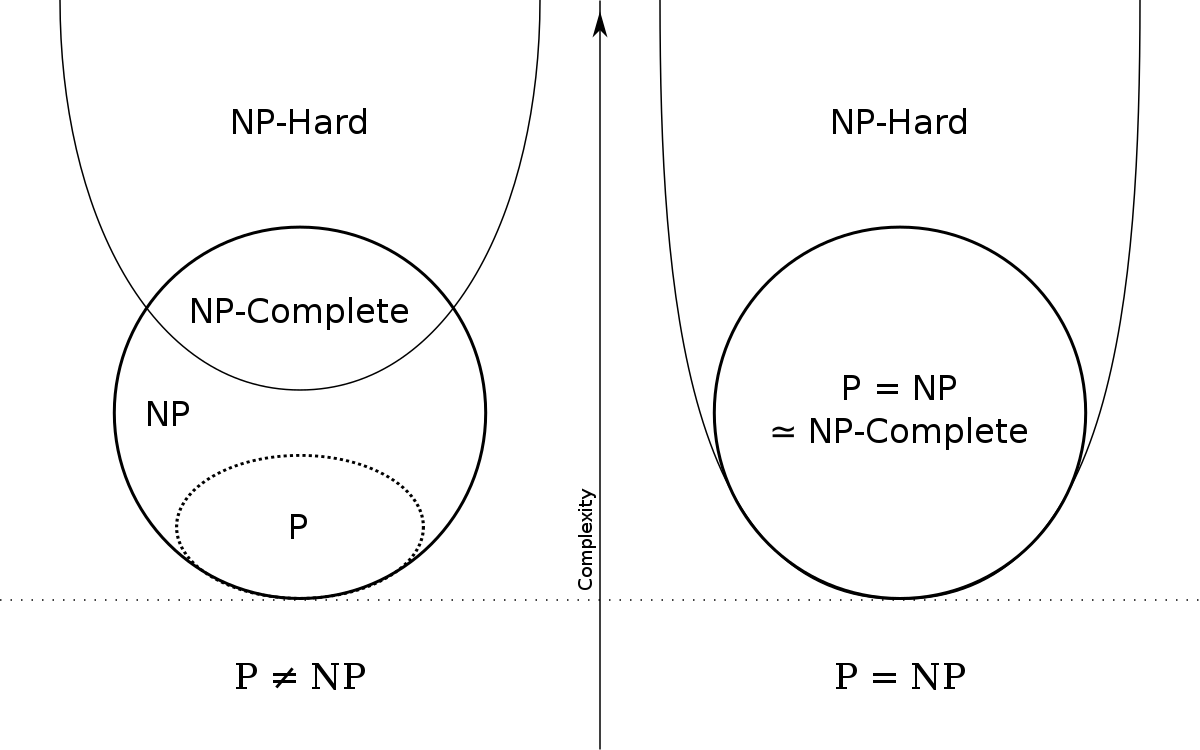
\includegraphics[scale = 0.3]{img/problem.png}
	\caption{Diagramma di \emph{Eulero Venn} per le classi di complessità}
	\label{fig:complexity}
\end{figure}
\begin{shaded}
	\textit{Tratto dagli appunti di Metodi Formali:}\\
	\begin{center}
		\textit{Si parla di isomorfismo quando due strutture complesse si possono
			applicare l'una sull'altra, cioè far corrispondere l'una all'altra, in modo
			tale che per ogni parte di una delle strutture ci sia una parte
			corrispondente nell'altra struttura; in questo contesto diciamo che due
			parti sono corrispondenti se hanno un ruolo simile nelle rispettive
		strutture.}
	\end{center}
	Diamo ora una definizione formale di isomorfismo tra sistemi di transizione
	etichettati, che possono quindi essere grafi dei casi o grafi dei casi
	sequenziali.
	\begin{definizione}
		Siano dati due sistemi di transizione etichettati:\\
		$A_1 = (S_1,E_1,T_1,s_{01})$ e $A_2 = (S_2 , E_2 , T_2 , s_{02})$.\\
		e siano date due \textbf{mappe biunivoche}:
		\begin{enumerate}
			\item $\alpha:S_1\to S_2$, ovvero che passa dagli stati del primo sistema a
			      quelli del secondo
			\item $\beta:E_1\to E_2$, ovvero che passa dagli eventi del primo sistema a
			      quelli del secondo
		\end{enumerate}
		allora:
		\[\langle \alpha,\beta\rangle:A_1= (S_1 , E_1 , T_1 ,s_{01})\to A_2 = (S_2 ,
			E_2 , T_2 , s_{02})\]
			è un \textbf{isomorfismo} sse:
			\begin{itemize}
				\item $\alpha(s_{01})=s_{02}$, ovvero l'immagine dello stato iniziale del
				      primo sistema coincide con lo stato iniziale del secondo
				\item $\forall s,s'\in S_1,\forall e\in E_1:\,(s,e,s')\in T_1
				      \Leftrightarrow (\alpha(s),\beta(e),\alpha(s'))\in T_2$ ovvero per ogni
				      coppia di stati del primo sistema, tra cui esiste un arco etichettato $e$,
				      vale che esiste un arco, etichettato con l'immagine di $e$, nel secondo
				      sistema che va dall'immagine del primo stato considerato del primo sistema
				      all'immagine del secondo stato considerato del secondo sistema, e viceversa
			\end{itemize}
			\end{definizione}
			\begin{definizione}
				Si definiscono due \textbf{sistemi equivalenti} sse hanno grafi dei casi
				sequenziali, e quindi di conseguenza anche grafi dei casi, \emph{isomorfi}.\\
				Due sistemi equivalenti accettano ed eseguono le stesse sequenze di eventi
			\end{definizione}
			\end{shaded}
			\section{Riduzioni polinomiali}
			Si hanno alcuni problemi che sono in grado di risolvere qualunque problema di
			decisione in \textbf{NP}. Serviranno prima le definizioni di \textbf{NP-hard} e
			\textbf{NP-complete}.\\
			Vediamo innanzitutto il problema \textit{independent-set} che ci aiuterà
			analisi.
			\begin{definizione}
				L'\textit{independent-set } di un grafo non orientato è un sottoinsieme
				$I\subseteq V$ tale che $\forall u,v\in I$ $(u,v)\not\in E$. Il problema
				\textit{ind\_set}, nella versione di ottimo, è quello di trovare
				l'\textit{independent-set} di cardinalità massima di un grafo non
				orientato. Nella versione di decisione $ind\_set_d$ si ha anche il parametro
				$k$ intero e si cerca se esiste un \textit{independent-set} di cardinalità
				uguale a $k$. L'\textit{independent-set} di cardinalità massima può essere
				usato come ``certificato''.
			\end{definizione}
			Questo problema è legato alla \textit{copertura dei vertici}, infatti sappiamo
			che se dall'insieme dei vertici togliamo un sottoinsieme di minima copertura
			troviamo un \textit{independent-set} di cardinalità massima perché sto facendo
			il complemento di un insieme di copertura di cardinalità minima, infatti tra i
			vertici non nell'insieme di copertura di cardinalità minima, ovvero nel
			complemento, non posso avere un arco per definizione e quindi se il primo è di
			cardinalità minima allora il secondo, che è l'\textit{independent-set}, è di
			cardinalità massima. Infatti i vertici nella copertura sono vertici che toccano
			tutti gli archi.\\
			Dal punto di vista delle applicazioni pratiche questi problemi si prestano allo
			studio, per esempio, delle telecomunicazioni.
			\begin{proof}
				Dimostriamo che $ind\_set_d$ è \textbf{NP}, infatti esiste un algoritmo $A$
				che in costo polinomiale prende in ingresso il grafo, $k$, e un
				``certificato'' $y$ e i vertici in $y$, che sono vertici di un
				\textit{independent\_set} per il grafo $G$ di cardinalità $k$. L'algoritmo
				verifica che $y$ è un \textit{independent-set} e il costo della verifica è
				quadratico su $|y|$, ovvero $|y|^2$ che nel caso peggiore è $|V|^2$. So anche
				che, per l'input $x$, $O(|x|)=O(|E|+|V|)=O(|V^2|+|V|)$ nel caso peggiore,
				quindi il tempo di verifica è \textbf{polinomiale}.
			\end{proof}
			\begin{definizione}
				Vediamo ora il problema di \textbf{soddisfacibilità} $SAT$. Questo problema
				prende in input una formula booleana $\phi$ in \textbf{forma normale congiunta
					(CNF)}, ovvero che ha una congiunzione ($\land$) come legame tra le
				\textbf{clausole}. Una clausola è un $\lor$ di \textbf{letterali}, ovvero di
				variabili booleane $x_i$ o $\neg x_i$. In output ho se la forma sia
				soddisfacibile o meno. 
				\begin{esempio}
					Prendo 3 variabili, $x_1,x_2,x_3$. Creo i letterali  $x_1,x_2,x_3$ e anche
					$\neg x_1,\neg x_2,\neg x_3$. Creo quindi le clausole $c_1=x_1\lor x_2$,
					$c_2=x_1\lor \neg x_2$ e $c_3=x_1\lor \neg x_2$. Definisco quindi la CNF
					$\phi$:
										    
					\[\phi=(x_1\lor x_2)\land (x_1\lor \neg x_2)\land
						(x_1\lor \neg x_2)=c_1\land c_2\land c_3\]
						Quindi in ogni clausola almeno un letterale deve essere vero, cosicché tutte
						le clausole siano vere rendendo vera la CNF.\\
						Avendo due letterali a clausola si è definito un $2SAT$.
						\end{esempio}
						Il numero di letterali $k$ che compongono la clausola definsice un problema
						$kSAT$. Si ha che $2SAT\in P$ ma con $k>2$ si ha che $kSAT\in NP$ (in
						realtà è in \textbf{NP-hard})
						\end{definizione}
						\begin{definizione}
							Definiamo un problema \textbf{NP-hard} come un problema difficile almeno
							quanto un problema \textbf{NP}. Ogni che problema $A$ in \textbf{NP} può
							essere risolto con un chiamata di procedura a $B$, che è un problema
							\textbf{NP-hard} a cui tutti gli altri ``chiedono aiuto'' per trovare una
							soluzione. \\
							Ad esempio \textit{vertex-cover} è un problema \textbf{NP-hard} e quindi posso
							risolvere ogni problema $A$ in \textbf{NP} con il problema
							\textit{vertex-cover} $B$.\\
							Trasformo quindi l'input $w$ di $A$ in un input
							$f(w)$ per $B$ in tempo polinomiale. La risposta di $B$ con input $f(w)$ è la
							stessa che $A$ da su input $w$.\\
							Non tutti i problemi \textbf{NP-hard} sono dentro la classe \textbf{NP}
						\end{definizione}
						\begin{definizione}
							Definiamo quindi il concetto di \textbf{riduzione}, rappresentato in figura
							\ref{fig:rid}.\\
							La riduzione è la trasformazione dell'input di $w$ in $A$ in un input $f(w)$
							per $B$, in tempo polinomiale. La risposta di $B$ con input $f(w)$ è la stessa
							che $A$ da su input $w$.\\
							Si ha che $A$ si riduce polinomialmente a $B$, e si scrive:
							\[A\leq_p B\]
							se $\exists\,f$ tale che:
							\[w \in L_A\mbox{ sse } f(w)\in L_B\]
							con $f$ calcolabile in tempo polinomiale, infatti il calcolo di $f(w)$ è
							$=(|w|^p)$, con $p\in\mathbb{N}$ per semplicità. Non devo introdurre una
							complessità superiore nel contesto di confronto tra problemi (??).\\ 
							\begin{figure}
								\centering
																    
								\psscalebox{0.9 0.9} % Change this value to rescale the drawing.
								{
									\begin{pspicture}(0,-2.8)(15.0,2.8)
										\definecolor{colour1}{rgb}{0.34901962,0.6627451,0.3019608}
										\definecolor{colour0}{rgb}{0.8784314,0.20392157,0.20392157}
										\definecolor{colour2}{rgb}{0.3254902,0.38039216,0.99607843}
										\psframe[linecolor=colour1, linewidth=0.04, dimen=outer]
										(13.52,2.8)(1.52,-2.8)
										\psframe[linecolor=colour0, linewidth=0.04, dimen=outer]
										(6.32,1.2)(2.72,-1.2)
										\psframe[linecolor=colour0, linewidth=0.04, dimen=outer]
										(6.32,1.2)(2.72,-1.2)
										\psframe[linecolor=colour2, linewidth=0.04, dimen=outer]
										(11.52,1.2)(7.92,-1.2)
										\psline[linecolor=black, linewidth=0.04, arrowsize=0.05291667cm 2.0,
										arrowlength=1.4,arrowinset=0.0]{->}(6.32,0.0)(7.92,0.0)
										\psline[linecolor=black, linewidth=0.04, arrowsize=0.05291667cm 2.0,
										arrowlength=1.4,arrowinset=0.0]{->}(0.72,0.0)(2.72,0.0)
										\psline[linecolor=black, linewidth=0.04, arrowsize=0.05291667cm 2.0,
										arrowlength=1.4,arrowinset=0.0]{->}(11.52,0.4)(14.32,0.4)
										\psline[linecolor=black, linewidth=0.04, arrowsize=0.05291667cm 2.0,
										arrowlength=1.4,arrowinset=0.0]{->}(11.52,-0.4)(14.32,-0.4)
										\rput[bl](3.7,1.3){Riduzione}
										\rput[bl](0.0,-0.14){$w$}
										\rput[bl](4.1,-0.08){$f(w)$}
										\rput[bl](9.42,-0.08){$B$}
										\rput[bl](12.26,0.6){yes}
										\rput[bl](14.42,0.25){yes}
										\rput[bl](12.34,-0.74){no}
										\rput[bl](14.42,-0.5){no}
										\rput[bl](9.24,1.3){$SAT$}
										\rput[bl](6.72,0.4){$f(w)$}
									\end{pspicture}
								}
								\caption{Rappresentazione grafica della riduzione}
								\label{fig:rid}
							\end{figure}
							Ogni problema $A$ che in \textbf{NP} può essere risolto con una chiamata di
							procedura a $B$, quindi posso risolvere ogni problema $A\in NP$ con
							\textit{vertex-cover}, essendo esso un problema \textbf{NP-hard}.
														  
						\end{definizione}
						\begin{definizione}
							$B$ è \textbf{NP-hard} sse $\forall A\in NP$ $A$ si riduce a $B$ in tempo
							polinomiale:
							\[A\leq_p B,\,\,\forall A\]
							Un problema $NP-hard$ può non essere in $NP$, in quanto potrebbe non avere un
							``certificato'' per consentire la verifica in tempo polinomiale.
						\end{definizione}
						\begin{definizione}
							Un problema \textbf{NP-hard} e anche \textbf{NP} si dice che il problema è
							\textbf{NP-complete} 
						\end{definizione}
						$kSAT$ è il primo problema che si è dimostrato essere anche
						\textbf{NP-complete}.
						\begin{esempio}
							Vediamo un esempio di riduzione, rappresentata in figura \ref{fig:ride}:
							\[3SAT\leq_p ind\_set_d\]
							arrivando e alla conclusione che $ind\_set_d$ è \textbf{NP-completo}.\\
							\begin{figure}
								\centering
																    
								\psscalebox{0.9 0.9} % Change this value to rescale the drawing.
								{
									\begin{pspicture}(0,-2.8)(15.0,2.8)
										\definecolor{colour1}{rgb}{0.34901962,0.6627451,0.3019608}
										\definecolor{colour0}{rgb}{0.8784314,0.20392157,0.20392157}
										\definecolor{colour2}{rgb}{0.3254902,0.38039216,0.99607843}
										\psframe[linecolor=colour1, linewidth=0.04, dimen=outer]
										(13.52,2.8)(1.52,-2.8)
										\psframe[linecolor=colour0, linewidth=0.04, dimen=outer]
										(6.32,1.2)(2.72,-1.2)
										\psframe[linecolor=colour0, linewidth=0.04, dimen=outer]
										(6.32,1.2)(2.72,-1.2)
										\psframe[linecolor=colour2, linewidth=0.04, dimen=outer]
										(11.52,1.2)(7.92,-1.2)
										\psline[linecolor=black, linewidth=0.04, arrowsize=0.05291667cm 2.0,
										arrowlength=1.4,arrowinset=0.0]{->}(6.32,0.0)(7.92,0.0)
										\psline[linecolor=black, linewidth=0.04, arrowsize=0.05291667cm 2.0,
										arrowlength=1.4,arrowinset=0.0]{->}(0.72,0.0)(2.72,0.0)
										\psline[linecolor=black, linewidth=0.04, arrowsize=0.05291667cm 2.0,
										arrowlength=1.4,arrowinset=0.0]{->}(11.52,0.4)(14.32,0.4)
										\psline[linecolor=black, linewidth=0.04, arrowsize=0.05291667cm 2.0,
										arrowlength=1.4,arrowinset=0.0]{->}(11.52,-0.4)(14.32,-0.4)
										\rput[bl](3.7,1.3){Riduzione}
										\rput[bl](0.35,-0.15){$\phi$}
										\rput[bl](4.1,-0.08){$f(\phi)$}
										\rput[bl](9.42,-0.08){$B$}
										\rput[bl](14.42,0.25){1}
										\rput[bl](14.42,-0.5){0}
										\rput[bl](9.0,1.3){$ind\_set_d$}
										\rput[bl](6.85,0.2){$G_\phi$}
									\end{pspicture}
								}
								\caption{Rappresentazione grafica del'esempio \ref{es:1}}
								\label{fig:ride}
							\end{figure}
							e vediamo che $\phi$ è soddisfacibile sse $G_\phi$ ha un
							\textit{independent-set} di dimensione $k=|\phi|$, con $|\phi|$ pari al numero
							di clausole della formula.\\
							Costruisco quindi un grafo che ha un vertice per ogni letterale della
							clausola. Collego i tre letterale della clausola ottenendo un
							``triangolo'', detto \textit{gadget}, che rappresenta una clausola. Infine
							collego ogni letterale al suo negato.
							\newpage
							Quindi per la formula:
							\[\phi=(\neg x_1\lor x_2\lor x_3)\land(x_1\lor \neg x_2\lor x_3)\land(\neg
								x_1\lor x_2\lor x_4)\]
								avrò il grafo $G_\phi$ che codifica la formula $\phi$:
								\begin{figure}[H]
									\centering
									\psscalebox{1.0 1.0} % Change this value to rescale the drawing.
									{
										\begin{pspicture}(0,-1.5798438)(12.92,1.5798438)
											\pscircle[linecolor=black, linewidth=0.04, fillstyle=solid,
											fillcolor=black, dimen=outer](1.6,0.9050586){0.4}
											\pscircle[linecolor=black, linewidth=0.04, fillstyle=solid,
											fillcolor=black, dimen=outer](0.4,-0.6949414){0.4}
											\pscircle[linecolor=black, linewidth=0.04, fillstyle=solid,
											fillcolor=black, dimen=outer](2.8,-0.6949414){0.4}
											\psline[linecolor=black, linewidth=0.02](1.6,0.5050586)(2.4,-0.6949414)
											\psline[linecolor=black, linewidth=0.02](1.6,0.5050586)(0.8,-0.6949414)
											\psline[linecolor=black, linewidth=0.02](0.8,-0.6949414)(2.4,-0.6949414)
											\rput[bl](1.2,1.3050586){$\neg x_1$}
											\rput[bl](2.6,-1.4949414){$x_3$}
											\rput[bl](0.2,-1.4949414){$x_2$}
											\pscircle[linecolor=black, linewidth=0.04, fillstyle=solid,
											fillcolor=black, dimen=outer](6.4,0.9050586){0.4}
											\pscircle[linecolor=black, linewidth=0.04, fillstyle=solid,
											fillcolor=black, dimen=outer](5.2,-0.6949414){0.4}
											\pscircle[linecolor=black, linewidth=0.04, fillstyle=solid,
											fillcolor=black, dimen=outer](7.6,-0.6949414){0.4}
											\psline[linecolor=black, linewidth=0.02](6.4,0.5050586)(7.2,-0.6949414)
											\psline[linecolor=black, linewidth=0.02](6.4,0.5050586)(5.6,-0.6949414)
											\psline[linecolor=black, linewidth=0.02](5.6,-0.6949414)(7.2,-0.6949414)
											\rput[bl](6,1.3050586){$\neg x_2$}
											\rput[bl](7.4,-1.4949414){$x_3$}
											\rput[bl](5.0,-1.4949414){$x_1$}
											\pscircle[linecolor=black, linewidth=0.04, fillstyle=solid,
											fillcolor=black, dimen=outer](11.2,0.9050586){0.4}
											\pscircle[linecolor=black, linewidth=0.04, fillstyle=solid,
											fillcolor=black, dimen=outer](10.0,-0.6949414){0.4}
											\pscircle[linecolor=black, linewidth=0.04, fillstyle=solid,
											fillcolor=black, dimen=outer](12.4,-0.6949414){0.4}
											\psline[linecolor=black,linewidth=0.02](11.2,0.5050586)(12.0,-0.6949414)
											\psline[linecolor=black,linewidth=0.02](11.2,0.5050586)(10.4,-0.6949414)
											\psline[linecolor=black,linewidth=0.02]
											(10.4,-0.6949414)(12.0,-0.6949414)
											\rput[bl](10.8,1.3050586){$\neg x_1$}
											\rput[bl](12.2,-1.4949414){$x_4$}
											\rput[bl](9.8,-1.4949414){$x_2$}
											\psline[linecolor=black, linewidth=0.02](0.8,-0.6949414)(6.0,0.9050586)
											\psline[linecolor=black, linewidth=0.02](2.0,0.9050586)(4.8,-0.6949414)
											\psline[linecolor=black, linewidth=0.02](5.6,-0.6949414)(10.8,0.9050586)
											\psline[linecolor=black, linewidth=0.02](6.8,0.9050586)(9.6,-0.6949414)
										\end{pspicture}
									}
									\label{es:1}
								\end{figure}
								Quindi un \textbf{gadget} è una rappresentazione dell'input del problema $A$
								di partenza e ogni \textbf{gadget} rappresenta una clausola.\\
								Ricordiamo che $\phi$ è soddisfacibile sse esiste un assegnamento delle
								variabili della formula tale per cui almeno un letterale di ogni clausola è
								vero. Nel grafo relativo alla formula lego quindi un letterale ad ogni suo
								complemento al fine di poter identificare i valori di verità e avendo il
								calcolo di \textit{independent-set} (per la \textbf{riduzione}) prendo uno
								solo degli estremi di un arco, e quindi uno solo tra $x_i$ e $\neg x_i$,
								codificando l'assegnamento di verità. Il concetto di \textbf{riduzione} è
								quindi ritrovabile nella capacità di rappresentare un problema in un'altra
								forma, studiabile con un altro algoritmo.
								\begin{proof}
									Indichiamo con $A$ $3SAT$ e con $B$ \textit{independent-set}.\\
									Effettuiamo quindi la prova finale, la dimostrazione vera e propria. A
									questo livello di comprensione abbiamo dimostrato
									l'esistenza della funzione $f$, che trasforma $\phi$ (ovvero l'input di $A$)
									in $\langle G, k\rangle$, ovvero l'input di $B$, e che essa è in tempo
									polinomiale. Abbiamo quindi che $w\in L_A$ sse $f(w)\in L_B$. Se $\phi$ è
									vera allora esiste un \textit{independent-set} di dimensione $k$ per
									$\langle G, k\rangle$.\\ 
									Nell'\,''altro verso'' abbiamo che se esiste un \textit{independent-set} di
									dimensione $k$ per $\langle G, k\rangle$ allora $\phi$ è vera. Dimostrare
									questi due ``versi'' equivale a dimostrare la riduzione.\\
									Il \textbf{primo verso} si dimostra dicendo che dato un assegnamento di
									verità si seleziona un letterale vero da ogni triangolo. Questi letterali
									veri scelti formano l'\textit{independent-set} $S$, che ha dimensione
									$k$. Questo può accadere sse $\phi$ è vera, infatti per ogni clausola $c_i$
									$\exists \,\,l_{ij}$, letterale, che rende vera $c_i$, a questo punto tale
									letterale è un vertice del triangolo, ovvero del gadget $g_{c_i}$, (mi basta
									infatti un letterale vero per triangolo) e, poiché
									tutte le clausole sono vere, ho la scelta di $k$ vertici se $k$ è il numero
									delle clausole. Esiste quindi un \textit{independent-set} di dimensione
									$k$.\\
									Per questo si potrebbe fare una \textbf{dimostrazione per costruzione},
									ovvero se rendo vera $c_y$ con $l_y$ significa che la variabile $x_i$ può
									essere usata o come 1 o come 0 nell'assegnamento di verità in un altro
									letterale $l_z$, che rende vera la clausola $c_z$. Ma $x_i$, se già usata,
									non posso più usarla con valore opposto a quello scelto per $c_y$ e quindi
									non esiste un arco di collegamento tra $l_y$ e $l_z$.\\
									Si può dimostrare anche per \textbf{assurdo}. Se esiste un arco tra i due
									letterali $l_z$ e $l_y$ che rendono vere le clausole $c_z$ e $c_y$,
									allora ottengo una contraddizione sugli assegnamenti di verità, asserendo
									che i due letterali sono uno la negazione dell'altro ma entrambi sono
									veri, per poter rendere vere le clausole. 
									\\
									\\
									Il \textbf{secondo verso} si dimostra dicendo che, dato un
									\textit{independent-set} 
									$S$ di dimensione $k$, $S$ deve contenere un vertice per triangolo. Ponendo
									quindi i letterali contenuti in $S$ come veri si ottiene un assegnamento di
									verità che è \textbf{consistente} e tutte le clausole sono soddisfatte.
									Quindi se esiste un \textit{independent-set} di dimensione $k$ allora trovo
									un assegnamento alle variabili $x_i,\,\,\forall \,\,1\ldots n$ che rende
									vera $\phi$, ovvero assegno 0 o 1 a ciascuna variabile (ovviamente o 1 o 0,
									non entrambi). Se esiste l'\textit{independent-set} di dimensione $k$ pari
									al numero delle clausole, allora per ogni gadget $g_{c_i}$,
									che rappresenta una clausola, esiste un vertice nel gadget che si trova
									anche nell'\textit{independent-set}, quindi esiste un letterale, per ogni
									clausola $c_i$ tale che non è collegato ad un altro letterale
									dell'\textit{independent-set}, ovvero non è collegato ad un altro letterale
									di un'altra clausola (ovvero ho un nodo per gadget che non ha un arco verso
									un nodo di un altro gadget). Quindi per ogni letterale vedo la variabile che
									rende vero il letterale e con il valore dato alla variabile costruisco
									l'assegnamento o 0 o 1 a quella variabile (se $l_i=\neg x_j$ allora
									$x_j=0$ e se $l_i= x_j$ allora $x_j=1$). Trovo quindi l'assegnamento delle
									variabili che è di verità per $\phi$, dimostrando quindi che $\phi$ è vera.
								\end{proof}
								\end{esempio}
								Siccome $3SAT$ è \textbf{NP-complete} allora anche \textit{independent-set} è
								\textbf{NP-complete}, infatti:
								\[\forall\,\, A_{\in NP}\leq_p 3SAT\leq_p \mbox{ \textit{independent-set}}\]
								in quanto la riduzione $\leq_p$ è \textbf{transitiva}, e quindi:
								\[\forall\,\, A_{\in NP}\leq_p \mbox{ \textit{independent-set}}\in NP\]
								\begin{definizione}
									Se un problema $\Pi$ \textbf{NP-complete} è in \textbf{P} allora si può dire
									$P=NP$, implicando che ogni problema $A\in NP$ è risolvibile da $\Pi\in P$.
									Questa cosa non è stata ancora dimostrata (e probabilmente si riuscirà
									a dimostrare l'opposto).
								\end{definizione}
								\begin{proof}
									Per ogni problema $A$ in \textbf{NP} so che $A\leq_p \Pi$, ovvero $\Pi$ è una
									procedura che risolve $A$, con trasformazione dell'input $x$ di $A$ nell'input
									$f(x)$ di $\Pi$, con $f(x)$ calcolabile in tempo polinomiale.\\
									Assumendo quindi che $\Pi\in P$ allora anche ogni $A\in P$, e quindi $NP=P$.
								\end{proof}
								\begin{definizione}
									La riduzione polinomiale è transitiva. Ovvero se $A\leq_p B$ e $B\leq_p C$
									allora:
									\[A\leq_p C\]
								\end{definizione}
								\begin{proof}
									Infatti $A\leq_p B$ implica l'esistenza di $f$ tale che $x\in L_A$ sse
									$f(x)=L_B$. Ugualmente $B\leq_p C$ implica l'esistenza di $g$ tale che $x\in
									L_B$ sse $g(x)=L_C$.\\
									Devo dimostrare che $\exists\,\,f'$ tale che $x\in L_A$ sse $f'(x)\in
									L_C$. Per ottenere $f'$ compongo $f$ e $g$. Assumendo che $x$ appartiene
									all'input di ha compongo le funzioni, quindi ho che $f'=g\circ f$,
									e ho che $x\in L_A$ e che $f(x)\in L_B$ (quindi $f(x)$ è un input per $B$) ma
									quindi $g(f(x))\in L_C$ (quindi $g(f(x))$ è un input per $C$). Ho quindi
									dimostrato la transitività.\\
									Se $f$ e $g$ sono costruibili in tempo polinomiale, la prima sulla dimensione
									di $x$ e la seconda su quella di $f(x)$, allora anche $f'=g\circ f$
									è costruibile in tempo polinomiale, proporzionalmente alla cardinalità di $x$.
								\end{proof}
								Quindi per dimostrare che un problema $\Pi'$ è \textbf{NP-hard} devo ridurre
								$\Pi'$ ad un problema qualsiasi \textbf{NP-hard} (in base alla somiglianza del
								problema), sapendo che $\forall A\in NP$ $A$ si riduce ad un problema
								\textbf{NP-hard}, come $SAT$.\\
								In modo equivalente per dire che è un problema è \textbf{NP-complete} faccio
								quanto fatto per \textbf{NP-hard} ma devo aggiungere che esso sia in $NP$,
								dovendo quindi aggiungere il ``certificato''.
								% immagine slide 6(definizione cook)
								\begin{definizione}
									Si ha che $SAT\leq_p 3SAT$
								\end{definizione}
								\begin{proof}
									\textbf{Dimostrazione solo parziale, solo l'inizio è stato fatto in aula.\\}
										Prendo una $\phi$ con $k\geq 4$ letterali. Ogni clausola deve diventare una
										clausola con al più 3 letterali (introducendo nuovi letterali ogni volta che
										viene negato uno). 
										\end{proof}
										\subsection{Problema set-cover}
										Questo problema si applica bene allo studio, nel campo delle telecomunicazioni,
										dei ripetitori e dello studio della copertura per reti mobili.
										\begin{definizione}
											Dato un universo $U$ di $n$ elementi sia $S=\{S_1,\ldots,S_M\}$ una collezione
											di sottoinsiemi di $U$. Sia anche data una funzione di costo
											$c:S\to\mathbb{Q}^+$. Il problema \textbf{set-cover} consiste nel trovare una
											collezione $C$ di sottoinsiemi di $S$ di costo minimo che copra tutti gli
											elementi di $U$.
										\end{definizione}
										\begin{esempio}
											Se ho $U=\{1,2,3,4,5\}$, $S_1=\{1,2,3\}$, $S_2=\{2,3\}$, $S_3=\{4,5\}$ e
											$S_4=\{1,2,4\}$, con $S=\bigcup S_i$ . Per praticità assumo costo
											uniforme, ovvero che  $c_1=c_2=c_3=c_4=1$.\\
											Quindi la soluzione $C$ è $\{S_1,S_3\}$, in quanto questi due insiemi coprono
											tutti gli elementi di $U$, con costo pari a $5$ (che è il minimo che posso
											avere).
										\end{esempio}
										\begin{definizione}
											Qualora il costo sia uniforme allora il \textbf{set-cover} diventa la ricerca
											di una sotto-collezione che copra tutti gli elementi di $U$ con minima
											dimensione.
										\end{definizione}
																				
										\begin{definizione}
											\textit{set-cover}, nella versione decisionale e nella
											versione con peso uniforme, è \textbf{NP-complete} (quindi se esiste una
											collezione $C$ di sottoinsiemi di $S$ 
											la cui unione sia $U$ con cardinalità minore uguale di $k$).
										\end{definizione}
										\begin{proof}
											Posso facilmente dimostrare che $|C|\leq k$ in tempo polinomiale e che
											l'unione degli insieme di $C$ include tutti gli elementi di $U$, in
											tempo polinomiale su $|U|$. Posso aggiungere anche un ``certificato'', nella
											forma di una collezione che copre tutto $U$ (e quindi la verifica è in tempo
											polinomiale sulla dimensione del ``certificato'' più quella di $U$). Quindi
											\textbf{set-cover} è in \textbf{NP}.\\
											Per dimostrare che \textbf{set-cover} è \textbf{NP-hard} dimostro che:
											\[\mbox{vertex-cover} \leq_p \mbox{set-cover}\]
											ovvero uso un problema che so già essere \textbf{NP-hard}, appunto
											\textit{vertex-cover} (avendo già dimostrato che $\forall A\in NP, \,\,A\leq_p
											\mbox{vertex-cover}$, dimostrando che \textit{set-cover} dimostra tutti i
											problemi in \textbf{NP}).\\
											Faccio vedere che posso usare \textit{set-cover} per dimostrare
											\textit{vertex-cover}.\\
											Devo quindi trasformare un'istanza di \textit{vertex-cover} $C=\langle
											G=(V,E), j\rangle$ in un'istanza $C'$ di \textit{set-cover}, in tempo
											polinomiale, tale che $C$ è soddisfacibile sse $C'$ è soddisfacibile.\\
											Procedo quindi con la trasformazione. Pongo innanzitutto $U=E$. Per quanto
											riguarda la collezione $S$ procedo nel seguente modo. Etichetto i vertici in
											$V$ da $1$ a $n$. A questo punto $S_i$ diventa l'insieme degli archi incidenti
											al vertice $i$-simo. A questo punto basta porre $k=j$ per concludere la
											costruzione polinomiale dell'istanza di \textit{set-cover}.\\
											In poche parole ciascun arco è un elemento di $U$ e ciascun vertice è un
											insieme di $S$.\\
											Vediamo anche la dimostrazione formale che \textit{vertex-cover} risponde
											``yes'', per $j$, sse istanza di \textit{set-cover} risponde ``yes'' per
											$k=j$.\\
											Innanzitutto se \textit{vertex-cover} risponde ``yes'' per $j$ allora trovo
											una collezione di \textit{set-cover} buona di cardinalità $j$. Suppongo
											infatti $G$ ha una copertura C di al più $j$ vertici e quindi $C$ corrisponde
											ad una collezione di $C'$ di sottoinsiemi $U$. Poiché assumo $k=j$ allora
											$|C'|\leq k$. Inoltre $C'$ copre tutti gli elementi di $U$ coprendo tutti gli
											archi di $G$, in quanto ogni elemento di $U$ è un arco in $G$. Poiché $C$ è
											una copertura, almeno un estremo dell’arco è in $C$  e quindi l’arco è in un
											insieme di $C'$.\\
											Dimostriamo anche l'altro verso della dimostrazione, ovvero devo garantire
											l'esistenza della copertura. Suppongo di avere un set cover $C'$ di dimensione
											$k$. Dato che ad ogni insieme di $C'$ ho associato un vertice in $G$ allora
											$|C|=|C'|\leq k=j$. Inoltre, $C$ è una copertura di $G$ poiché $C'$ è un
											set-cover, poiché, preso un arco $e$ ho che $e\in U$ e quindi $C'$ deve
											contenere almeno un insieme che contiene $e$ e tale insieme è quello che
											corrisponde ai nodi che sono estremi di $e$. Quindi $C$ deve contenere almeno
											un estremo di $e$. Quindi posso concludere dicendo che $C$ è copertura di $G$.
										\end{proof}
										Si continua la ricerca di una dimostrazioni di \textbf{NP-completezza}, ambito
										di studio nato dopo la scoperta di Cook di $SAT\in$ \textbf{NP-complete}.\\
										Partiamo ricordando che:
										\begin{definizione}
											Se $B$ è un problema tale che $A\leq_p B$, con $A$
											\textbf{NP-hard} (o ovviamente anche \textbf{NP-complete}), allora $B$ è
											\textbf{NP-hard} e se inoltre $B\in NP$ allora $B$ è \textbf{NP-complete}.  
										\end{definizione}
										\begin{proof}
											Con la transitività della riduzione $\leq_p$ si ha che $\forall\pi\in
											NP,\,\,\, \pi\leq_p A$ e quindi $A$ è \textbf{NP-hard}. Inoltre avendo
											$A\leq_p B$ ho che  $\pi\leq_p B$ e quindi $B$ è \textbf{NP-hard}, inoltre,
											avendo $B\in NP$, ho che è \textbf{NP-complete}
										\end{proof}
																				
																				
										\subsection{Problemi di ottimizzazione}
										\subsubsection{Clique-problem}
										\begin{definizione}
											Definisco \textbf{clique (\textup{cricca})} di un grafo non orientato
											$G=(V,E)$ come un sottoinsieme $V'\subseteq V$ di vertici tale che:
											\[\forall \,v_1,v_2\in V' (v_1,v_2)\in E\]
											quindi un sottoinsieme di vertici con solo vertici collegati da un arco.
										\end{definizione}
										Definisco quindi il problema.
										\begin{definizione}
											Il \textbf{clique-problem} è un problema di ottimizzazione (nel
											dettaglio di massimo) in cui si cerca la \textbf{clique} di dimensione massima
											di un grafo (ovvero $|V'|$ è massimo). Nella versione decisionale chiedo se
											esiste una \textbf{clique} di dimensione $k$.\\
											Il problema è \textbf{NP-complete}
										\end{definizione}
										\begin{proof}
											Dimostriamo che sia \textbf{NP-complete} (nella versione decisionale). Cerco
											quindi un algoritmo 
											polinomiale, con``certificato''. Uso quindi un insieme $V'\subseteq V$ come
											vertici della \textbf{clique} come ``certificato'' per il grafo in input. Per
											verificare che $V'$ è una \textbf{clique} controllo che:
											\[\forall\,v_1,v_2\in    V' (v_1,v_2)\in E\]
											e questa verifica è polinomiale, infatti è $O(|V'|^2)$ e
											quindi è quadratico nella dimensione dell'input.\\
											Bisogna ora trovare un problema $A\in \mbox{NP-complete}$ tale che $A$ si
											riduce in tempo polinomiale al \textbf{clique-problem} (quindi
											\textbf{clique-problem} risolve $A$).  \\
											Notiamo che una \textbf{clique} è l'opposto di \textbf{independent-set}, che
											avevamo dimostrato tramite $3SAT$ (che può risolvere
											\textbf{independent-set}).\\
											Quindi per \textbf{clique-problem} provo ancora ad usare $3SAT$. Devo fare in
											modo che $\phi\in 3SAT$ sse il grafo $G_\phi$ ha una \textbf{clique} di
											dimensione uguale al numero di clausole di $\phi$. Quindi avendo $k$ clausole
											in $\phi$ avrò che ciascuna clausola sarà un gadget e da ogni gadget estrarrà
											un vertice che comporrà la \textbf{clique} di dimensione $k$.\\
											Il grafo $G_\phi$ è costruito come nel caso di \textit{independent-set} coi
											letterali come vertici.\\
											Bisogna studiare il collegamento tra tali vertici (che sarà diverso al caso di
											\textit{independent-set}, non avendo quindi i triangoli).\\
											Ipotizzo:
											\[\phi=c_1\land c_2\land c_3\]
											con:
											\[c_1=x_1\lor \neg x_2\lor \neg x_3\]
											\[c_2=\neg x_1\lor x_2\lor x_3\]
											\[c_3=x_1\lor x_2\lor x_3\]
											Per ogni clausola faccio i vertici per ogni letterale (distinti anche per lo
											stesso letterale, come nel caso di \textit{independent-set}).\\
											Per ora abbiamo vertici isolati e i tre vertici isolati di ogni clausola sono
											il gadget. A questo punto collego ogni letterale di ogni clausola con ogni
											altro letterale di ogni altra clausola (non della stessa) che non sia
											l'opposto, collegando quindi solo vertici \textbf{consistenti} (in quanto non
											potrei avere una \textbf{clique} connettendo due vertici non consistenti). Sto
											facendo esattamente l'opposto di \textit{independent-set}. 
											\begin{figure}
												\centering
												\psscalebox{0.9 0.9} % Change this value to rescale the drawing.
												{
													\begin{pspicture}(0,-4.3798437)(8.58,4.3798437)
														\definecolor{colour0}{rgb}{0.003921569,0.003921569,0.003921569}
														\pscircle[linecolor=black, linewidth=0.04,
														fillstyle=solid,fillcolor=colour0, dimen=outer](2.8,3.3050585){0.4}
														\pscircle[linecolor=black, linewidth=0.04,
														fillstyle=solid,fillcolor=colour0, dimen=outer](6.8,3.3050585){0.4}
														\pscircle[linecolor=black, linewidth=0.04,
														fillstyle=solid,fillcolor=colour0, dimen=outer](4.8,3.3050585){0.4}
														\pscircle[linecolor=black, linewidth=0.04,
														fillstyle=solid,fillcolor=colour0, dimen=outer](1.2,2.1050587){0.4}
														\pscircle[linecolor=black, linewidth=0.04,
														fillstyle=solid,fillcolor=colour0, dimen=outer](1.2,-1.8949414){0.4}
														\pscircle[linecolor=black, linewidth=0.04,
														fillstyle=solid,fillcolor=colour0, dimen=outer](1.2,0.105058596){0.4}
														\pscircle[linecolor=black, linewidth=0.04,
														fillstyle=solid,fillcolor=colour0, dimen=outer](2.8,-3.0949414){0.4}
														\pscircle[linecolor=black, linewidth=0.04,
														fillstyle=solid,fillcolor=colour0, dimen=outer](6.8,-3.0949414){0.4}
														\pscircle[linecolor=black, linewidth=0.04,
														fillstyle=solid,fillcolor=colour0, dimen=outer](4.8,-3.0949414){0.4}
														\rput[bl](2.65,3.9050587){$x_1$}
														\rput[bl](4.4,3.9050587){$\neg x_2$}
														\rput[bl](6.4,3.9050587){$\neg x_3$}
														\rput[bl](0.0,2.0050587){$\neg x_1$}
														\rput[bl](0.2,0.0405058596){$x_2$}
														\rput[bl](0.2,-2.0949414){$x_3$}
														\rput[bl](2.63,-3.8949413){$x_1$}
														\rput[bl](4.63,-3.8949413){$x_2$}
														\rput[bl](6.63,-3.8949413){$x_3$}
														\psline[linecolor=black, linewidth=0.04](4.8,2.9050586)(2.8,-2.6949415)
														\psline[linecolor=black, linewidth=0.04](4.8,2.9050586)(6.8,-2.6949415)
														\psline[linecolor=black, linewidth=0.04](4.8,2.9050586)(1.6,2.1050587)
														\psline[linecolor=black, linewidth=0.04](4.8,2.9050586)(1.6,-1.8949414)
														\psline[linecolor=black, linewidth=0.04](6.8,2.9050586)(4.8,-2.6949415)
														\psline[linecolor=black, linewidth=0.04](6.8,2.9050586)(2.8,-2.6949415)
														\psline[linecolor=black, linewidth=0.04](6.8,2.9050586)(1.6,0.105058596)
														\psline[linecolor=black, linewidth=0.04](6.8,2.9050586)(1.6,2.1050587)
														\psline[linecolor=black, linewidth=0.04](1.6,2.1050587)(4.8,-2.6949415)
														\psline[linecolor=black, linewidth=0.04](1.6,2.1050587)(6.8,-2.6949415)
														\psline[linecolor=black, linewidth=0.04]
														(1.6,0.105058596)(2.8,-2.6949415)
														\psline[linecolor=black, linewidth=0.04]
														(1.6,0.105058596)(4.8,-2.6949415)
														\psline[linecolor=black, linewidth=0.04]
														(1.6,0.105058596)(6.8,-2.6949415)
														\psline[linecolor=black, linewidth=0.04](1.6,-1.8949414)(2.8,-2.6949415)
														\psline[linecolor=black, linewidth=0.04](1.6,-1.8949414)(4.8,-2.6949415)
														\psline[linecolor=black, linewidth=0.04](1.6,-1.8949414)(6.8,-2.6949415)
														\psline[linecolor=black, linewidth=0.04](2.8,2.9050586)(2.8,-2.6949415)
														\psline[linecolor=black, linewidth=0.04](2.8,2.9050586)(4.8,-2.6949415)
														\psline[linecolor=black, linewidth=0.04](2.8,2.9050586)(6.8,-2.6949415)
														\psline[linecolor=black, linewidth=0.04](2.8,2.9050586)(1.6,0.105058596)
														\psline[linecolor=black, linewidth=0.04](2.8,2.9050586)(1.6,-1.8949414)
													\end{pspicture}
												}
												\caption{Grafo $G_\phi$ per \textbf{clique-problem}, con le due righe di
												nodi e la colonna che rappresentano i tre gadget}
												\label{fig:cli}
											\end{figure}
											Costruito il grafo $G_\phi$ cerco almeno una \textbf{clique} di dimensione 3
											per $3SAT$. Non potrò mai avere più di un letterale per clausola nella
											\textbf{clique} non essendo tra loro collegati.\\
											Passare da $\phi$ a $G_\phi$ ha costo polinomiale in tempo, ottenendo quindi
											istanza, in tempo polinomiale. \\
											Inoltre bisogna dimostrare che se $\phi$ ha un assegnamento che la rende vera
											allora esiste una \textbf{clique} per $G_\phi$ di dimensione $k$. Se $\phi$ è
											vera allora per ogni clausola $c_r$ esiste almeno un letterale che è vero e
											assumiamo che tale letterale sia $l_{i}^r=1$. Questo letterale è associato al
											vertice $v_i^r$. Quindi data la clausola $c_i$, vera per il letterale $l_j^i$
											allora costruisco l'insieme dei vertici $V'\subseteq V$ tale che sia formato
											da quei singoli vertici corrispondenti ai singoli letterali veri. Questo $V'$
											è una \textbf{clique} infatti avrò solo letterali ``collegabili'' nel grafo
											(non essendo vero che un letterale sia vero e contemporaneamente falso, cosa
											che comporterebbe l'assenza dell'arco). Ho solo archi tra letterali
											consistenti tra loro e quindi, per costruzione, esiste l'arco tra i vertici
											corrispondenti ($\forall\, u,v\in V'$).\\
											Inoltre bisogna dimostrare che, se esiste una \textbf{clique} di dimensione
											$k$, allora $\phi$ è vera e quindi le $K$ clausole sono tutte vere. \\
											Per ogni vertice di $v_{it}\in V'$ se appartiene al gadget della clausola
											$c_t$ rendo vero il letterale associato (o falso se esso è negato). A questo
											punto rendo vera ogni clausola rendendo vero almeno un suo letterale e quindi
											so di ottenere un assegnamento di verità per $\phi$ in quanto i letterali, per
											come sono stati definiti, sono consistenti.
											\\ \textbf{sistemare formalismi}
										\end{proof}
										\begin{proof}
											Dimostriamo che la riduzione del problema \textit{clique}, che sappiamo essere
											\textbf{NP-complete}, è in tempo polinomiale.\\ 
											Vediamo che la trasformazione della formula $\phi$ di $3SAT$ nel grafo
											$G_\phi$ è una riduzione in tempo polinomiale.\\
											Dato un assegnamento che rende vera $\phi$, che ha $k$ clausole, dobbiamo
											costruire una \textit{clique} per $G_\phi$ che abbia $k$ vertici. Ciascuna
											clausola $c_{r}$ ha almeno un letterale $l_{i}^r$ che ha assegnato il valore 1,
											$\top$. Ciascun letterale $l_{i}^r$ corrisponde ad un vertice
											$v_{i}^r$. Costruiamo $V'$ insieme di vertici per ogni letterale $l_i^r$ vero
											per ogni clausola $c_r$. Dimostriamo che $V'$ è una \textit{clique}. Si ha che
											per ogni coppia $v_i^r,v_j^s\in V',\,\,r\neq s$ (due vertici rappresentanti
											due letterali di due clausole diverse) abbiamo che $(v_i^r,v_j^s)\in
											E$ essendo entrambi i letterali veri e,per costruzione, sono consistenti, cioè
											uno non è l'opposto dell'altro.\\
											Vediamo l'altro verso.\\
											Supponiamo che $G_\phi$ abbia una \textit{clique} $V'$ di dimensione $k$ e
											bisogna vedere se $\phi$ è vera. Sappiamo che $V'$, per costruzione ha
											esattamente un solo vertice per ogni clausola, $v_i^r$ per la clausola
											$c_r$. Prendo quindi il letterale corrispondente $l_i^r$ e assegno a tale
											letterale il valore 1 (se negato 0). Quindi so che il letterale complemento di
											$l_i^r$ non verrà usato per rendere vera una clausola perché il vertice
											$v_i^r$ non è collegato con un arco ad un vertice che rappresenta il
											c0complemento di $l_i^r$. Quindi riesco a costruire un assegnamento di verità
											\textit{consistente} (ovvero ogni variabile è presa come $x_i=1$ oppure
											$x_i=0$ ma non entrambi i valori sono usati) per $\phi$.
										\end{proof}
										Si può dimostrare che:
										\[clique\leq_p vertex\_cover\]
										\[independent\_set\leq_p vertex\_cover\]
										\[vertex\_cover\leq_p independent\_set\]
										\[vertex\_cover\leq_p clique\]
										Infatti vale il seguente definizione:
										\begin{definizione}
											Se ho che:
											\[A\leq_p B\]
											e $A,B\in \mbox{NP-complete}$, allora:
											\[B\leq_p A\]
										\end{definizione}
										\begin{proof}
											Infatti, siccome $B$ è in \textbf{NP-complete} allora è anche in \textbf{NP},
											allora: 
											\[B\leq_p A\]
											Ma posso fare lo stesso discorso con $A$, essendo in \textbf{NP-complete} e
											quindi sono interscambiabili e quindi:
											\[A\leq_p B\]
										\end{proof}
										I problemi \textbf{NP-complete} richiedono quindi una soluzione efficiente.\\
										Bisogna quindi pensare ad algoritmi di approssimazione, algoritmi polinomiali
										con ``garanzia'', ovvero \textbf{euristiche} (ovvero un qualcosa che funziona in
										pratica) per il problema. Non si ha quindi una soluzione esatta al problema,
										l'euristica non fornisce una soluzione esatta.\\
										L'obiettivo è quindi quello di risolvere i problemi \textbf{NP-complete}.
										\begin{definizione}
											Definiamo un \textbf{problema di ottimizzazione}, dato un problema $\Pi$ e
											un'istanza $x$, come la ricerca di un ottimo di $x$, detto $opt(x)$. Il costo
											di una soluzione ammissibile su $x$ calcolato da un algoritmo $A$ per il
											problema $\Pi$ è indicato con $A(x)$ (che quindi è il costo della soluzione
											calcolato da $A$).\\
																						  
											Si cerca quindi la soluzione, tra tutte quelle di $\Pi$, che massimizza o
											minimizza una funzione costo (appunto $opt(x)$). Non sappiamo chi calcoli
											questo costo.
										\end{definizione}
										\begin{definizione}
											Definiamo un \textbf{algoritmo $\varepsilon$-approssimato} per un problema
											$\Pi$ è un 
											algoritmo $A$ polinomiale che restituisce una soluzione ammissibile che dista
											da quella ottima di un fattore $\varepsilon$.\\
											Se $\Pi$ è un \textbf{problema di minimo} allora:
											\[A(x)\leq \varepsilon\cdot opt(x), \mbox{ \textnormal{con} }\varepsilon>1\]
											Si raggiunge quindi un valore più grande del minimo, di una quantità fissata
											$\varepsilon$. Devo quindi garantire che non sia troppo grande, tramite
											$\varepsilon$.\\
											Si ha quindi che:
											\[\frac{A(x)}{opt(x)}\leq \varepsilon\]
											L'algoritmo lavora in tempo polinomiale e risolve in modo approssimato
											problemi $\Pi$ \textbf{NP-completi}. Se avessi $\varepsilon=1$ avrei la
											soluzione ottima, ma non sarebbe possibile in quanto avrei un algoritmo
											polinomiale per un algoritmo \textbf{NP-completo}.\\
											Se $\Pi$ è un \textbf{problema di massimo} allora:
											\[A(x)\geq \varepsilon\cdot opt(x), \mbox{ \textnormal{con} }0<\varepsilon<1\]
											In quanto raggiungo una soluzione più piccola del massimo ma devo garantire
											che non sia troppo piccola, tramite $\varepsilon$. $\varepsilon\cdot opt(x)$ è
											infatti una ``frazione'' dell'ottimo.\\
											Si ha quindi che:
											\[\frac{A(x)}{opt(x)}\geq \varepsilon\Longrightarrow\frac{opt(x)}{A(x)}\leq
												\frac{1}{\varepsilon}\]
												A seconda del problema devo trovare un $\varepsilon$, che viene fissata
												costante per ogni input (e quindi è indipendente dall'input stesso e dalla sua
												dimensione) che serve da ``garanzia''. So quindi che $A(x)$, ovvero il costo
												della soluzione approssimata ammissibile calcolata da $A$, in tempo
												polinomiale, si rapporta a $opt(x)$, calcolata dall'algoritmo esatto in tempo
												esponenziale (se fosse polinomiale si avrebbe $P=NP$), tramite una distanza
												$\varepsilon$ (da un alto è un $\limsup$ e dall'altro un $\liminf$).\\
												Tipicamente si ha come valore tipico per $\varepsilon$ 2, avendo quindi
												una \textbf{2-approssimazione}, in quanto facilmente dimostrabile.
												\end{definizione}
												\begin{esempio}
													Prendiamo \textit{vertex-cover} nella versione di ottimo. Dato $G=(V,E)$ ha
													come soluzione ammissibile una copertura di vertici per $G$. Il costo di una
													soluzione è la cardinalità di $V'$, se $V'$ è una soluzione ammissibile.\\
													Il costo ottimo di \textit{vertex-cover} invece è la minima cardinalità di
													$V'$.
												\end{esempio}
												\begin{definizione}
													Si ha il cosiddetto \textbf{approximation ratio} $r$ dicendo che:
													\[\max\left\{\frac{A(x)}{opt(x)},\frac{opt(x)}{A(x)}\right\}\leq r,\mbox{
															\textnormal{con} }r>1\] 
														Il primo caso copre il caso di minimo mentre il secondo caso copre il massimo.
														\end{definizione}
														\textbf{Non tutti i problemi ammettono una \textit{r}-approssimazione, per
															\textit{r} costante}.\\
														Ci sono problemi infatti dove il calcolo di:
														\[\max\left\{\frac{A(x)}{opt(x)},\frac{opt(x)}{A(x)}\right\}\leq \rho(n)\]
														per una certa funzione $\rho$,con $|x|=n$,
														ovvero il massimo dipende dalla
														dimensione dell'input, non avendo quindi più un $r$ costante. La dimensione del
														problema influisce sulla capacità di approssimazione e degradano all'aumentare
														della dimensione. Si ha, per esempio, $\rho(n)=\log n$.\\
														Per capire $\varepsilon$ fornisco un'euristica $A$ per il problema e provo a
														dimostrare, senza conoscere l'ottimo (quindi per ogni possibile input), che in
														ogni caso:
														\[\frac{A(x)}{opt(x)}\leq \varepsilon\]
														dimostrando che si ha una $\varepsilon$-approssimazione (non sempre è
														dimostrabile o perlomeno per alcuni problemi si è ancora riusciti).
														\begin{definizione}
															Esiste $A$ polinomiale per \textit{vertex-cover} che è 2-approssimante,
															quindi:
															\[\frac{A(x)}{opt(x)}\leq 2\]
														\end{definizione}
														\begin{proof}
															Prendo il grafo $G=(V,E)$.\\
															Cerco un $A$ che calcoli in tempo polinomiale una soluzione ammissibile,
															ovvero una copertura di vertici del grafo. Si sceglie che $A$ non deve essere
															un \textit{algoritmo greedy}.\\
															Prendo quindi un arco del grafo $e=(u,v)\in E$. Inizio a costruire una
															copertura $C$, all'inizio vuota ($C=\emptyset$), che ora diventa, aggiungendo
															i due vertici:
															\[C=C\cup\{u,v\}\]
															Inoltre rimuovo dall'insieme degli archi $E$ tutti gli archi che hanno un
															estremo nell'attuale copertura $C$, e quindi nel nostro caso in $u$ o $v$.\\
															Procedo quindi iterativamente costruendo $C$ fermandomi quando $E$ risulti
															vuoto, ovvero fino a che $E=\emptyset$.\\
															È quindi una 2-approssimazione in quanto al massimo posso prendere il doppio
															dei vertici per fare la copertura, infatti, per costruzione, seleziono ogni
															volta archi che non hanno estremi in comune. Per ognuno di questi archi scelti
															devo prendere i due estremi, quindi ho $2\cdot k$ vertici in $C$ per $k$ archi
															e quindi:
															\[A(x)=2\cdot k\]
															Ma di $opt(x)$ so che nel casi migliore prende esattamente un estremo per ogni
															arco scelto dall'algoritmo, e quindi per archi che non hanno estremi in
															comune. Quindi nel caso migliore:
															\[opt(x)\geq k\]
															Dato che stiamo cercando di minimizzare, quindi $k$ è il \textit{lower bound} e
															quindi:
															\[\frac{A(x)}{opt(x)}\leq\frac{2k}{k}\leq 2\]
															Come volevasi dimostrare.
														\end{proof}
														\begin{algorithm}
															\begin{algorithmic}
																\Function{VCApprox}{$G=(V,E)$}
																\State $C\gets\emptyset$
																\State $E'\gets E$
																\While {$E'\neq \emptyset$}
																\State $\mbox{let }(u,v)\in E'$
																\State $C\gets C\cup \{u,v\}$
																\For {$\mbox{every }(u,z)\in E'\land\mbox{ every } (v,z')\in E'$}
																\State $\mbox{delete } (u,z),(v,z') \mbox{ from } E'$
																\EndFor
																\EndWhile
																\State \textbf{return} $C$
																\EndFunction
															\end{algorithmic}
															\caption{Algoritmo di vertex-cover approssimato}
														\end{algorithm}
														\newpage
														L'idea della 2-approssimazione è quella che si cerca un limite inferiore
														all'ottimo per il problema, ad esempio, appunto, \textit{vertex-cover}. Si ha
														che:
														\[opt(x)\geq k\]
														con $k$ che è il $\liminf$ mentre $opt(x)$ è la dimensione dell'ottimo su
														istanza X, nel caso di \textit{vertex-cover} ho $x=G=(V,E)$. Sviluppo quindi un
														algoritmo polinomiale che produce una soluzione ammissibile per il problema e
														tale che abbia costo di tale soluzione sia $\varepsilon$ volte il limite
														inferiore dell'ottimo, con $\varepsilon>1$:
														\[A(x)=\varepsilon\cdot \liminf,\,\,\,\varepsilon>1\]
														Inoltre ho che:
														\[A(x)\leq \varepsilon\cdot k,\,\,\,\varepsilon>1\]
														e quindi:
														\[\frac{A(x)}{opt(x)}\leq\frac{\varepsilon\cdot k}{k}\leq \varepsilon\]
														avendo quindi una $\varepsilon$-approssimazione.\\
														Nel caso di \textit{vertex-cover} costruisco un \textbf{matching perfetto},
														selezionando archi del grafo che non condividono i vertici estremi. Utilizzo
														quindi tutti i vertici, per il \textit{matching perfetto}. Una copertura minima
														del grafo deve per forza ottenere esattamente un vertice per ogni arco di
														matching, perché non hanno estremi in comune. Quindi il limite inferiore
														dell'ottimo è il numero di archi del matching (visto che ho un vertice per
														arco):
														\[opt(x)\geq |E_{matching}|\]
														Posso usare una tecnica greedy per costruire il matching, mettendo nelle
														soluzioni ammissibili entrambi gli estremi di ogni arco, per l'ammissibilità,
														per poi fare la rimozione degli archi incidenti.\\
														L'algoritmo $A$ quindi costruisce in modo greedy (o meglio ``in modo
														incrementale'', incrementantalmente) un matching per $G$ così:
														\\
														prende un arco $e_i$ e rimuove tutti gli archi incidenti agli estremi
														di $e_i$ inserendo nella soluzione ammissibile entrambi gli estremi di
														$e_i$. Sicuramente l'arco successivo scritto da $A$ non condivide estremi con
														$e_i$.\\
														L'unico problema è che $A(x)$ ha dimensione doppia rispetto al numero di archi:
														\[A(x)=2\cdot |E_{matching}|\]
														del matching mentre:
														\[opt(x)\geq |E_{matching}|\]
														avendo quindi la 2-approssimazione.\\
														\subsection{Problemi NP-hard non NP}
														Vediamo un algoritmo \textbf{NP-hard} che non è in \textbf{NP}, o meglio che
														ancora non sia dimostrato esserlo.
														Si congettura che non sia possibile che tutti i problemi \textbf{NP-hard} siano
														nella classe \textbf{NP}.\\ 
														Si parla comunque di problemi di decisione decidibili.\\
														Non posso al momento attuale dimostrare che un problema \textbf{NP-hard} non sia
														in \textbf{NP} ma si hanno problemi per cui non si riesce a mostrare che siano
														in \textbf{NP}, ovvero nessuno è riuscito a costruire un algoritmo con
														``certificato'' per questi problemi. Si ricorda la figura
														\ref{fig:complexity}.
														\subsubsection{Quantified boolean formula problem}
														Un esempio è decidere se una formula $\phi$ con \textit{quantificatori} è
														vera. Per questo problema \textbf{NP-hard} non esiste un algoritmo con
														certificato, non ancora perlomeno.\\
														Una \textbf{Quantified Boolean Formula (\textit{QBF})} $\phi$ è una formula
														proposizionale con dei \textit{quantificatori}, ovvero della forma:
														\[\phi=Q_{1p_1}Q_{2p_2}\ldots Q_{1n_n}\]
														Con un quantificatore $Q_{ip_i}$ relativi alle proposizioni $p_i$.\\
														Si ha:
														\[Q_i\in\{\forall,\exists\}\]
														\begin{esempio}
															Vediamo un esempio di QBF:
															\[\forall\, p_1\exists\,p_2\,\exists\, p_3(p_1\to(p_1\land p_3))\]
														\end{esempio}
														Decidere se la formula $\phi$ è vera è un problema \textbf{PSPACE-complete},
														ovvero un problema che si risolve con spazio polinomiale rispetto all'input $x$,
														ma al momento attuale nessuno ha mostrato che il problema QBF appartiene a
														\textbf{NP}.\\
														Diversi problemi possono essere espressi in QBF (come ad esempio le mosse degli
														scacchi) ma questi per ora sono tutti in tempo esponenziale.\\
														Aumentando il numero di quantificatori mi sposto in una nuova gerarchia, in un
														contesto di gerarchie infinite dove ad ogni aumento di un quantificatore
														corrisponde una classe di complessità nuova che contiene tutte quelle
														precedenti.\\
														Noi sappiamo che:
														\[P\subseteq NP\subseteq PSPACE=NPSPACE\subseteq EXPTIME\subseteq NEXPTIME\]
														La classe PSPACE è la classe di tutti i problemi accettati da un Turing Machine
														in spazio polinomiale. La classe\textbf{EXPTIME} ha tempo esponenziale e
														\textbf{NEXPTIME} se il problema è risolvibile da una Turing Machine non
														deterministica.
														\begin{definizione}
															Un problema $\Pi$ è \textbf{complete} per una classe di complessità $k$ sse 
															$\Pi\in k$ ed è \textbf{difficile} per quella classe.\\
															SI hanno:
															\begin{itemize}
																\item \textbf{NP-complete}
																\item \textbf{NPSPACE-complete}
															\end{itemize}
														\end{definizione}
														\section{Complessità parametrica}
														La \textbf{complessità parametrica} è stata introdotta negli anni novanta e
														viene studiata molto in ambito di \textbf{bioinformatica} e studio di
														\textbf{reti/grafi}.\\
														Un problema \textbf{NP-complete} posso dire che alcune istanze sembrano
														risolvibili in tempo polinomiale, fissando determinati parametri che
														caratterizzano l'istanza. Ad esempio prendo \textit{vertex-cover} con al più una
														certa dimensione $k$ in un grafo comunque molto complesso, magari con $10^8$
														nodi e $k$ fissato a un numero piccolo, tipo $5$. Non cerco quindi una minima
														copertura ma una di una certa dimensione, piccola. In questo caso, con $k$
														piccolo, un tempo esponenziale in $k$ è accettabile (esempio $2^5$ è
														accettabile).\\
														Mi serve quindi un algoritmo polinomiale sull'input ma esponenziale su $k$.
														\begin{definizione}
															Un problema decidibile $\Pi$ è \textbf{trattabile fissato il parametro, Fixed
																Parameter Tractable (\textit{FPT})}, con parametro $k$, sse esiste un
															algoritmo $A$, una costante $c$ e una funzione computabile $f$ tale che per
															tutti gli input $\langle x,k\rangle$ $A$ risolve $\Pi$ con tempo di calcolo:
															\[T(n) = f(k)\cdot|x|^c=f(k)\cdot n^c\]
															Si arriva quindi ad un $O(f(k)\cdot n^c)$ con $f$ esponenziale in $k$
															fissato. \\
															L'input diventa quindi $(x,k)$.
														\end{definizione}
														Quindi ho comunque un tempo polinomiale in $x$ ed esponenziale in $k$, $|x|^c\to
														2^k$. Divido quindi l'input in due dimensioni ed esprimo il tempo evidenziando
														i due parametri.\\
														Se avessi un algoritmo $A$, con input $x$, per un problema \textbf{NP-complete}
														avrei $2^{|x|}=2^n$ ma avendo in input $\langle x,k\rangle$ diventa polinomiale
														in $|x|=n$ ma esponenziale in $k$. Nella risposta quindi considero una parte
														limitata dell'input, per questo serve $k$ piccolo.\\
														Fissato $k$ ho una \textbf{soluzione esatta} e quindi gli algoritmi parametrici
														sono vantaggiosi rispetto agli algoritmi di approssimazione.\\
														Non tutti i problemi possono avere un problema parametrico associato.\\
														Queste tecniche vengono usate per trattare problemi \textbf{NP-hard},
														considerando problemi di ottimizzazione e non di decisione.
														\subsection{Vertex-cover parametrico}
														Prendendo \textit{vertex-cover} \textbf{decisionale} cerco una copertura di
														dimensione massima $k$. Ho quindi in input $\langle G=(V,E),k\rangle$ e trovo un
														algoritmo che decide se esiste tale copertura minima in tempo $T(n)$, in
														funzione di $n$ e $k$.\\
														Si ha il seguente definizione:
														\begin{definizione}
															Il problema vertex-cover $(G,k)$ è risolvibile in tempo $O(2^k\cdot |V|)$ dove
															$V$ è l'insieme dei vertici di $G$, con la costante che non dipende da $k$ e
															da $|V|$. Si ha quindi:
															\[O^*(f(x))=O(2^k\cdot |V|)\]
															Avendo $O^*$ che specifica indipendenza da $k$ e da $|V|$.
														\end{definizione}
														Si vuole quindi $s^{|V|}=2^k$.\\
														Si parte quindi cercando di costruire insiemi con al più $k$ vertici esplorando
														un albero binario di ricerca, sviluppandolo fino a profondità $2^k$, che avrà
														come foglie degli insiemi \textit{vertex-cover} di dimensione $k$.\\
														Si quindi ricorre ai \textbf{Bounded search trees (\textit{alberi di ricerca
														limitati})}. Si costruisce quindi un albero binario di profondità $k$, con
														il numero di nodi che quindi cresce circa per $O(2^k)$ e che sono una copertura
														candidata. \\
														Si prende la radice $r$ dell'albero e dato l'arco $(u,v)\in E$ ho due figli di
														$r$, uno con $u$ e l’altro con $v$, costruisco quindi due figli a partire dalla
														radice. Questo si fa in quanto basta avere o $u$ o $v$ nella copertura e quindi
														separo le due situazioni possibili date dalla scelta di uno dei due
														estremi. Scelto un arco arco $(x,v)$ non coperto da $u$ e estendo il nodo di $u$
														collegandolo ad altri due nodi, uno con $\{u, v\}$ e uno con $\{u, x\}$ (fisso
														$k=3$): 
														\begin{center}
															\begin{tikzpicture}[shorten >=1pt,node distance=1.7cm,on grid,auto]
																\node[state, accepting] (q_0) {$r$};
																\node[state] (q_1) [below right=of q_0] {$\{v\}$};
																\node[state] (q_2) [below left=of q_0] {$\{u\}$};
																\path[->]
																(q_0) edge  node {$v$} (q_1)
																(q_0) edge  node [above left] {$u$} (q_2);
															\end{tikzpicture}
														\end{center}
														Proseguo poi via via con ulteriori archi che non sono coperti dai vertici
														foglia, etichettando gli archi dell'albero con l'identificativo del vertice che
														ho aggiunto. \\
														Aggiungo ad esempio $(x,v)$:
														\begin{center}
															\begin{tikzpicture}[shorten >=1pt,node distance=1.9cm,on grid,auto]
																\node[state, accepting] (q_0) {$r$};
																\node[state] (q_1) [below right=of q_0] {$\{v\}$};
																\node[state] (q_2) [below left=of q_0] {$\{u\}$};
																\node[state] (q_3) [below right=of q_2] {$\{u,v\}$};
																\node[state] (q_4) [below left=of q_2] {$\{u,x\}$};
																\path[->]
																(q_0) edge  node {$v$} (q_1)
																(q_0) edge  node [above left] {$u$} (q_2)
																(q_2) edge  node {$v$} (q_3)
																(q_2) edge  node [above left] {$x$} (q_4);
															\end{tikzpicture}
														\end{center}
														aggiungo poi $(z,t)$:
														\begin{center}
															\begin{tikzpicture}[shorten >=1pt,node distance=2.3cm,on grid,auto]
																\node[state, accepting] (q_0) {$r$};
																\node[state] (q_1) [below right=of q_0] {$\{v\}$};
																\node[state] (q_2) [below left=of q_0] {$\{u\}$};
																\node[state] (q_3) [below right=of q_2] {$\{u,v\}$};
																\node[state] (q_4) [below left=of q_2] {$\{u,x\}$};
																\node[state] (q_5) [below right=of q_4] {$\{u,x, z\}$};
																\node[state] (q_6) [below left=of q_4] {$\{u,x,t\}$};
																\path[->]
																(q_0) edge  node {$v$} (q_1)
																(q_0) edge  node [above left] {$u$} (q_2)
																(q_2) edge  node {$v$} (q_3)
																(q_2) edge  node [above left] {$x$} (q_4)
																(q_4) edge  node {$z$} (q_5)
																(q_4) edge  node [above left] {$x$} (q_6)
																; 
															\end{tikzpicture}
														\end{center}
														(mi fermo che sono a $k=3$)\\
														Scriviamo il processo formalmente.\\
														Ricorsivamente si ha che sia $S$ l'insieme che etichetta un vertice, scelgo
														$(u',v')$ in E che non è coperto da S, quindi creo due figli con etichetta $S +
														{u'}$ e $S + {v'}$. Si ha che se c'è un percorso di lunghezza $k$ da $r$ ad un
														nodo $S$ che è una copertura per $G$ allora non c’è bisogno di esplorare oltre
														l’albero, facendo quindi il \textbf{bound}, ovvero il taglio dell'albero. \\
														Ovviamente ogni split non esclude che i due risultati coprano lo stesso
														insieme. La scelta di ordine di archi da esplorare è casuale.\\
														Ovviamente se ad altezza $k$ non trovo una copertura minima significa che non
														esiste una copertura di $k$ nodi.\\
														Vediamo un esempio:
														\begin{esempio}
															Sia dato il grafo:
															\begin{center}
																\begin{tikzpicture}[shorten >=1pt,node distance=2.3cm,on grid,auto]
																	\node[state] (q_0) {$2$};
																	\node[state] (q_1) [below right=of q_0] {$3$};
																	\node[state] (q_2) [below left=of q_0] {$1$};
																	\node[state] (q_3) [below left=of q_2] {$5$};
																	\node[state] (q_4) [below left=of q_1] {$4$};
																	\node[state] (q_5) [below right=of q_1] {$6$};
																	\path[-]
																	(q_0) edge  node {} (q_1)
																	(q_0) edge  node {} (q_2)
																	(q_2) edge  node {} (q_1)
																	(q_2) edge  node {} (q_3)
																	(q_2) edge  node {} (q_5)
																	(q_0) edge  node {} (q_1)
																	(q_1) edge  node {} (q_4)
																	(q_1) edge  node {} (q_3)
																	; 
																\end{tikzpicture}
															\end{center}
															Scelgo di imporre $k=2$.\\
															Inizio con l'arco $(1,2)$ (la scelta è casuale):
															\begin{center}
																\begin{tikzpicture}[shorten >=1pt,node distance=1.7cm,on grid,auto]
																	\node[state, accepting] (q_0) {$r$};
																	\node[state] (q_1) [below right=of q_0] {$\{2\}$};
																	\node[state] (q_2) [below left=of q_0] {$\{1\}$};
																	\path[->]
																	(q_0) edge  node {$2$} (q_1)
																	(q_0) edge  node [above left] {$1$} (q_2);
																\end{tikzpicture}
															\end{center}
															Scelgo poi $(2,3)$:
															\begin{center}
																\begin{tikzpicture}[shorten >=1pt,node distance=1.9cm,on grid,auto]
																	\node[state, accepting] (q_0) {$r$};
																	\node[state] (q_1) [below right=of q_0] {$\{2\}$};
																	\node[state] (q_2) [below left=of q_0] {$\{1\}$};
																	\node[state] (q_3) [below right=of q_2] {$\{1,3\}$};
																	\node[state] (q_4) [below left=of q_2] {$\{1,2\}$};
																	\path[->]
																	(q_0) edge  node {$2$} (q_1)
																	(q_0) edge  node [above left] {$1$} (q_2)
																	(q_2) edge  node {$3$} (q_3)
																	(q_2) edge  node [above left] {$2$} (q_4);
																\end{tikzpicture}
															\end{center}
															scelgo poi $(1,7)$
															\begin{center}
																\begin{tikzpicture}[shorten >=1pt,node distance=2.4cm,on grid,auto]
																	\node[state, accepting] (q_0) {$r$};
																	\node[state] (q_1) [below right=of q_0] {$\{2\}$};
																	\node[state] (q_2) [below left=of q_0] {$\{1\}$};
																	\node[state] (q_3) [below =of q_2] {$\{1,3\}$};
																	\node[state] (q_4) [left=of q_2] {$\{1,2\}$};
																	\node[state] (q_5) [right=of q_1] {$\{2,1\}$};
																	\node[state] (q_6) [below =of q_1] {$\{2,7\}$};
																	\path[->]
																	(q_0) edge  node {$2$} (q_1)
																	(q_0) edge  node [above left] {$1$} (q_2)
																	(q_2) edge  node {$3$} (q_3)
																	(q_2) edge  node [above] {$2$} (q_4)
																	(q_1) edge  node {$1$} (q_5)
																	(q_1) edge  node [left] {$7$} (q_6);
																\end{tikzpicture}
															\end{center}
															e mi fermo essendo a profondità 2.
															Tra le foglie cerco le coperture e noto che $\{1,3\}$ è effettivamente una
															copertura minima.
														\end{esempio}
														\textbf{su elearning appunti extra con algoritmo e calcolo dei tempi}.
														\subsection{TSP metrico}
														\begin{definizione}
															Definiamo \textbf{ciclo di Eulero} come un ciclo che tocca tutti gli archi
															del grafo una e una sola volta. Posso tornare allo stesso vertice e quindi i
															vertici hanno grado entrante pari a quello uscente (numero di archi entranti
															pari a quello di quelli uscenti):
															\[indegree=outdegree\]
														\end{definizione}
														Vediamo quindi un algoritmo parametrico per TSP. Il problema TSP consiste nella
														pratica nel trovare un \textbf{ciclo hamiltoniano} di costo minimo. Ricordiamo
														che un ciclo hamiltoniano è un ciclo semplice, non orientato, che passa per ogni
														nodo di $G$. Il costo del ciclo è pari alla somma dei costi dei suoi archi.\\ 
														Parliamo di \textbf{TSP simmetrico} se il grafo non è orientato, altrimenti è
														detto \textbf{TSP asimmetrico}. TSP è un problema \textbf{NP-hard}.\\
														Studiamo quindi un'euristica per TSP. Si definisce $w_{xy}$ come il peso
														dell'arco tra i nodi $x$ e $y$.\\
														Definiamo \textbf{TSP metrico} come un TSP dove vale la \textbf{distanza}
														``vera'', ovvero i costi sono attribuiti tramite la \textbf{disuguaglianza
															triangolare}. Si ha che $\forall(u,v)\in E$ $w_{uv}=0$ sse $u=v$. Inoltre,
														dati tre nodi distinti, vale appunto la disuguaglianza triangolare:
														\[w_{uv}\leq w_{uz}+w_{zv}\]
														e quindi $w$ introduce una semimetrica, che accettiamo come metrica.
														Applicando questo concetto ad un intero cammino posso dire che un arco tra due
														vertici ha costo sicuramente minore uguale di quello di un cammino tra i due
														archi (praticamente estendo ogni volta il conto facendo una serie di triangoli
														usando sempre la disuguaglianza triangolare).\\
														Una classe molto importante di metriche èquella delle metriche indotte dalle
														varie norme $\norm{\cdot}_p$:
														\[d_{\norm{\cdot}_p}(i,j)=\norm{i-j}_p=\left(\sum_{k=1}^m
															|i_k-j_k|^p\right)^{\frac{1}{p}}\]
															e al variare di $p$ si hanno varie metriche:
															\begin{itemize}
																\item \textbf{distanza di Manahattan} se $p=1$:
																      \[d_{\norm{\cdot}_1}(i,j)=\sum_{k=1}^m|i_k-j_k|\]
																\item \textbf{distanza Euclidea} se $p=2$:
																      \[d_{\norm{\cdot}_2}(i,j)=\left(\sum_{k=1}^m
																      	|i_k-j_k|^2\right)^{\frac{1}{2}}\]
																      	\item \textbf{distanza di Lagrange} se $p=\infty$:
																      	\[d_{\norm{\cdot}_\infty}(i,j)=\max_k\{|i_k-j_k\}\]
																      	\end{itemize}
																      	Per descrivere la 2-approssimazione, detta di \textbf{Christofides}, per TSP
																      	usiamo il ciclo di Eulero.
																      	\begin{definizione}
																      		Definiamo multigrafo come un grafo che prevede la possibilità di avere archi
																      		diversi tra due nodi (possono anche essere cappi).
																      	\end{definizione}
																      	\begin{definizione}[definizione di Eulero]
																      		Un (multi)grafo ammette un ciclo euleriano se e solo se è connesso e ogni nodo
																      		ha grado pari (quindi per un arco entrante ho un arco uscente).\\
																      		Un (multi) grafo connesso e con ogni nodo di grado pari è detto grafo
																      		euleriano. 
																      	\end{definizione}
																      	Esiste un algoritmo polinomiale per costruire un ciclo euleriano da un grafo,
																      	che se lo ammette è chiamato \textbf{grafo euleriano}. Si procede scomponendo il
																      	grafo in cicli che poi vengono fusi secondo un meccanismo che esclude archi già
																      	visitati.\\
																      																	      	
																      	Studiamo quindi l'\textbf{algoritmo di Christofides}. Viene dato in input un
																      	grafo $G=(V,E)$, non orientato, completo, con costi dati dalla funzione $c$ e
																      	dotato di semimetrica. 
																      	L'algoritmo trova un ciclo hamiltonianodi costo al piùdoppio rispetto al ciclo
																      	di costo minimo procedendo tramite alberi di copertura minima, ovvero:
																      	\begin{enumerate}
																      		\item si trova il minimo albero ricoprente $T$ di $G$, questo ha costo
																      		      polinomiale tramite l'\textbf{algoritmo di Prim}. Per questo problema
																      		      l’algoritmo greedy garantisce l’ottimo, basta infatti scegliere gli archi in
																      		      ordine di costo crescente ma saltando quelli che chiudono ciclo
																      		\item si raddoppia ogni arco di $T$ ottenendo un grafo euleriano
																      		\item si costruisce un ciclo euleriano $\epsilon$ di questo grafo, questo ha
																      		      costo polinomiale, basta infatti percorrere uno dopo l’altro tutti i cicli
																      		      ottenuti dai rami dell’albero 
																      		\item si visita $\epsilon$ partendo da un nodo iniziale $u$
																      		\item si costruisce una permutazione $\pi$ dei nodi $V$ di $G$
																      		      \textit{sequenziando i nodi} nell’ordine della loro prima apparizione in
																      		      $\epsilon$ nella visita (potrei avere comunque archi che accorciano il
																      		      percorso essendo $G$ completo (???)). 
																      		\item si restituisce il ciclo hamiltoniano $H$ associato a $\pi$
																      	\end{enumerate}
																      	In pratica si ha un'euristica che si dimostra essere 2-approssimante.\\
																      	Inoltre si ha che $c$ soddisfa la disuguaglianza triangolare (saltando dei nodi
																      	seguo delle scorciatoie) allora si ha che:
																      	\[c(H)\leq c(\epsilon)\]
																      	\begin{definizione}
																      		Sia $H^*$ il ciclo hamiltonianodi costo minimo, e sia $T$ l'albero di
																      		copertura minima di $G$ di costo minimo. Si ha quindi che:
																      		\[c(H^*)\geq c(T)\]
																      	\end{definizione}
																      	\begin{definizione}
																      		Sia $H^*$ il ciclo hamiltoniano di costo minimo, e sia $H$ il ciclo ritornato
																      		dall’algoritmo di Christofides, allora si ha che:
																      		\[c(H)\leq 2\cdot c(H^*)\]
																      		Avendo così la 2-approssimazione.
																      	\end{definizione}
																      	\begin{proof}
																      		Si ottiene quindi che $c(H)$ approssima la soluzione di minimo costo, che
																      		indichiamo con $c(H^*)$, avendo $H^*$ come il ciclo hamiltonianodi costo
																      		minimo. \\
																      		Si ha inoltre che, dato $c(T)$ come costo dell'albero di copertura:
																      		\[c(\epsilon)=2\cdot c(T)\]
																      		perché $\epsilon$ è il ciclo di eulero del grafo $G_T$ ottenuto duplicando gli
																      		archi di $T$ e $\epsilon$ attraversa una sola volta tutti gli archi di tale
																      		grafo:
																      		\[c(\epsilon)=c(\epsilon(G_T))=2\cdot c(T)\]
																      		Si può quindi anche dire che:
																      		\[c(T)\geq c(H^*)\]
																      		dato che $H^*$ è ottenuto da un certo albero $T'$, che non sappiamo se è di
																      		copertura minimo, a cui viene aggiunto un arco $e'$.
																      		Ma sappiamo che:
																      		\[c(T')\geq c(T)\]
																      		riassumendo un ciclo hamiltoniano ottimo è quindi costituito da un albero di
																      		copertura $T'$ (che non sappiamo se è di copertura minimo e quindi $c(T)\leq
																      		c(T')$ più un arco $e'$ che chiude l'albero ad un ciclo per cui: 
																      		\[c(H^*)\geq c(T')\]
																      		avendo che:
																      		\[c(H^*)=C(T')+c(e')\]
																      		A questo punto si ha:
																      		\[c(T)\leq c(T')\leq c(H^*)\]
																      		Sapendo quindi che:
																      		\[c(\epsilon)=2\cdot c(T)\]
																      		e che:
																      		\[2\cdot c(T)\leq 2\cdot c(H^*)\]
																      		e quindi si ottiene che:
																      		\[c(H)\leq c(\epsilon)\leq 2\cdot c(H^*)\]
																      		e quindi:
																      		\[c(H)\leq 2\cdot c(H^*)\]
																      		dimostrando la 2-approssimazione.
																      	\end{proof}
																      																	      	
																      	\begin{esempio}
																      		Partiamo da:
																      		\begin{figure}[H]
																      			\centering
																      			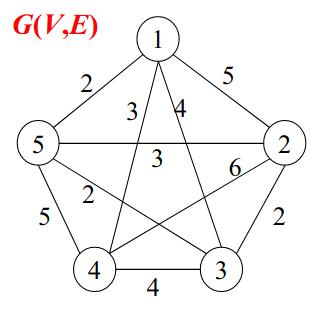
\includegraphics[scale = 0.4]{img/ch1.jpg}
																      		\end{figure}
																      		Procediamo con lo step 1, ottenendo $T$:
																      		\begin{figure}[H]
																      			\centering
																      			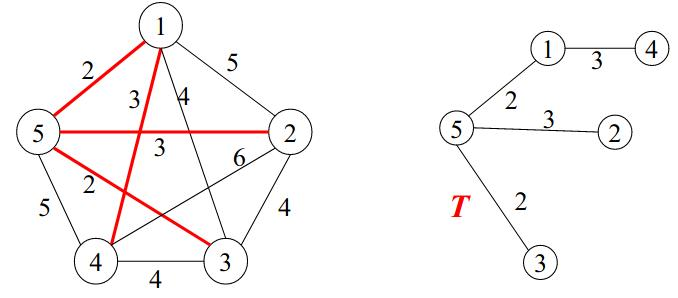
\includegraphics[scale = 0.4]{img/ch2.jpg}
																      		\end{figure}
																      		Procediamo con lo step 2, raddoppiando ogni arco di $T$:
																      		\begin{figure}[H]
																      			\centering
																      			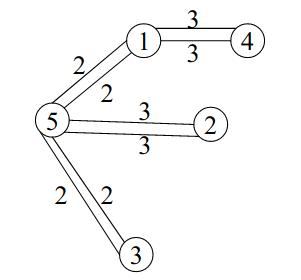
\includegraphics[scale = 0.4]{img/ch3.jpg}
																      		\end{figure}
																      		Procediamo con lo step 3, ottenendo $\epsilon$:
																      		\begin{figure}[H]
																      			\centering
																      			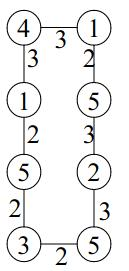
\includegraphics[scale = 0.4]{img/ch4.jpg}
																      		\end{figure}
																      		e con gli step 4 e 5 si ha:
																      		\begin{figure}[H]
																      			\centering
																      			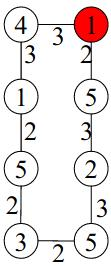
\includegraphics[scale = 0.4]{img/ch5.jpg}
																      		\end{figure}
																      		che deve essere ``letto'' in senso orario.\\
																      		Si ha quindi la sequenza di visita:
																      		\[\epsilon=\{1,5,2,5,3,5,1,4\}\]
																      		con la permutazione associata:
																      		\[\pi=\{1,5,2,3,4\}\]
																      		Si arriva quindi, con lo step 6, a:
																      		\begin{figure}[H]
																      			\centering
																      			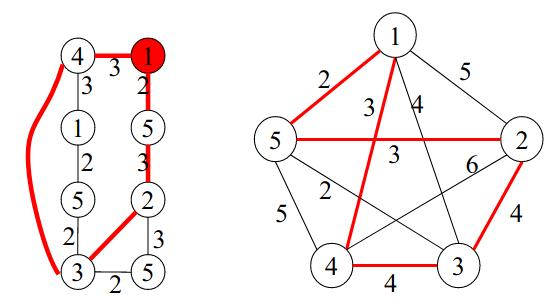
\includegraphics[scale = 0.4]{img/ch6.jpg}
																      		\end{figure}
																      		(avendo che comunque un arco tra due nodi che sostituisce un cammino tra quei
																      		nodi sicuramente costa meno o la più costa uguale, avendo la semimetrica)
																      	\end{esempio}
																      	L'\textbf{algoritmo di Christofides} trova quindi un'euristica cercando un
																      	\textit{lower bound}, tramite l'albero di copertura.\\
																      	\subsubsection{Cammino hamiltoniano e TSP}
																      	Abbiamo visto che il cammino hamiltoniano è un problema \textbf{NP-complete} e
																      	sappiamo che (si veda lezione nel capitolo sulle macchine di Turing,
																      	cronologicamente fatta prima):
																      	\[hamiltonianPath\leq_P TSP\]
																      	(aggiungendo gli archi mancanti con costo maggiore dell'unità)
																      	\begin{definizione}
																      		TSP (non metrico) non ha un'approssimazione costante a meno che $P=NP$.
																      	\end{definizione}
																      	\begin{proof}
																      		Sia $G=(V,E)$ il grafo in analisi su cui costruire il ciclo hamiltoniano.
																      		Costruiamo un
																      		$G'=(V', E', W)$ tale che:
																      		\[
																      			\begin{cases}
																      				w((u,v)) = 1\mbox{ sse } e=(u,v) \in E                            
																      				w(e)=\varepsilon\cdot|V|+1 \mbox{ altrimenti (pesando più di 1)} 
																      			\end{cases}
																      		\]
																      		Si assume quindi  di avere un algoritmo $\varepsilon$-approssimato.
																      		Si hanno due casi:
																      		\begin{enumerate}
																      			\item l'algoritmo restituisce un tour di costo $|V|$ e quindi esiste il
																      			      ciclo hamiltoniano
																      			\item l'algoritmo $A$ restituisce un tour con almeno un arco di costo
																      			      $\varepsilon\cdot|V|+1$ e quindi $A(x)>\varepsilon\cdot |V|$
																      		\end{enumerate}
																      		Ma per definizione di $\varepsilon$-approssimazione ho che:
																      		\[\varepsilon\cdot opt(x)\geq A(x)\]
																      		e quindi si ha che:
																      		\[opt(x)>\frac{A(x)}{\varepsilon}>|V|\]
																      		cioèil tour ottimoèdi costomaggiore di $|V|$ e quindi non esiste un ciclo
																      		hamiltoniano (non c’è modo di avere Un tour di costo $|V|$).\\
																      		Pertanto $A$ diventa un algoritmo per deciderese esiste o meno un
																      		cammino hamiltoniano dove $A$ è polinomiale cioè è nella classe
																      		P. L’algoritmo è fatto come segue:
																      		\begin{itemize}
																      			\item se $A(x)=|V|$ allora ho che $opt(x)=|V|$ ed esiste il ciclo
																      			      Hamiltoniano, altrimenti deve essere che $A(x)>\varepsilon\cdot |V|$ ma per
																      			      costruzione ho che $opt(x)>|V|$ e quindi non esiste il ciclo hamiltoniano ma
																      			      poiché il problema del ciclo hamiltoniano è in NP, ne consegue che P$=NP$,
																      			      dimostrando il definizione.
																      		\end{itemize}
																      	\end{proof}
																      	Esistono quindi problemi che non hanno approssimazione costante.\\
																      	Esistono anche problemi che hanno $\varepsilon$-approssimazione costante
																      	$\forall\,\varepsilon$ piccolo a piacere (si parla di \textbf{Polynomial time
																      		approximation scheme (\textit{PTAS})}). 
																      	\subsection{Closest string}
																      	\textbf{Fatta velocemente e sembra fuori esame}.\\
																      	In questo problema si ha in input una collezione di $k$ stringhe
																      	$s_1,\ldots,s_k$ di lunghezza $l$. Si ha anche un input $d$ e in output si ha
																      	una stringa $s$ tale che:
																      	\[d_H(s,s_j)\leq d,\,\,\,\forall\,j= 1,\ldots,k\]
																      	dove con $d_H(s,s')$ indichiamo la \textbf{distanza di Hamming} tra due stringhe
																      	$s$ e $s'$, ovvero il numero di simboli diversi tra esse.
																      	\begin{definizione}
																      		Closest string è risolvibile in tempo:
																      		\[O(d+1)^d|G|\]
																      		e se $d$ è piccolo, allora il tempo $O(d+1)^d$ è accettabile (esempio per
																      		distanza Hamming $d = 5$) anche quando l’input è molto grande  
																      	\end{definizione}
																      	\textbf{Dimostrazione extra su slide}.